\documentclass{article}[12pt,subeqn]

%\usepackage{fancyhdr}
%\pagestyle{fancy}
\usepackage{epsfig}
\usepackage{epstopdf}
%\usepackage[pdftex]{graphicx}
\usepackage{setspace}
\usepackage{framed}
\usepackage{lastpage}
\usepackage{amsmath}
\usepackage[utf8]{inputenc}
\title{The Twin Instrument: The Fertility Investment Tradeoff}
\author{Sonia Bhalotra\thanks{University of Bristol, \href{mailto:s.bhalotra@bristol.ac.uk}{s.bhalotra@bristol.ac.uk}.} \and Damian Clarke\thanks{The University of Oxford, \href{mailto:damian.clarke@economics.ox.ac.uk}{damian.clarke@economics.ox.ac.uk}.}}
\date{\today}

\setlength\topmargin{-0.575in}
%\setlength\headheight{15pt}
%\setlength\headwidth{6.05in}
\setlength\textheight{9in}
\setlength\textwidth{6.2in}
\setlength\oddsidemargin{0.18in}
\setlength\evensidemargin{-0.5in}
\setlength\parindent{0.25in}
\setlength\parskip{0.25in}

\usepackage{natbib}
\bibliographystyle{abbrvnat}
\bibpunct{(}{)}{;}{a}{,}{,}

\usepackage{hyperref}
\usepackage{nohyperref}
\usepackage{url}

\usepackage{lscape}
\usepackage{rotating}
\usepackage{multirow}
\usepackage{rotating,capt-of}
\usepackage{array}

%\usepackage{lineno}
%\usepackage[update,prepend]{epstopdf}

\usepackage[font=sc]{caption}

%NEW COMMANDS
\newcommand{\Lagr}{\mathcal{L}}
\newcommand{\vect}[1]{\mathbf{#1}}
\newcolumntype{P}[1]{>{\raggedright}p{#1\linewidth}}

\usepackage{appendix}
\usepackage{booktabs}
\usepackage{cleveref}

%\fancyhead{}
%\fancyfoot{}
%\fancyhead[L]{\textsc{Extended Essay}}
%\fancyhead[C]{\textsc{MSc. Economics for Development}}
%\fancyhead[R]{\textsc{Damian C. Clarke}}
%\fancyfoot[C]{\textsc{\thepage\ of  \pageref{LastPage}}}
%\fancyfoot[R]{\texttt{ \Large DRAFT}}



\begin{document}
%\linenumbers
\begin{spacing}{1.25}



\maketitle
\end{spacing}
\begin{spacing}{1.5}	

\begin{abstract}
The incidence of twins has been used to identify the impact of changes in fertility on measures of investment in children born prior to the twins, and the emerging consensus in this literature is that there is no evidence of a quantity-quality trade-off. We argue that the standard approach is flawed for two reasons. First, even if twin conception is random, bringing twins to term is a function of maternal health which is difficult to fully observe and which tends to be correlated with child quality, rendering the instrument invalid. Second, twins will only constitute a shock to family size if their occurrence takes family size across the desired level. The neglect of both of these considerations in the literature will tend to lead to under-estimation of the Q-Q trade-off and so could contribute to explaining the negative results in the literature. Using a large sample of microdata from developing countries, we show that a significant trade-off emerges upon correcting for these biases.
\end{abstract}
\newpage

\section{Introduction}
\label{scn:intro}
Twin studies since at least \citet{RosenzweigWolpin1980} have attempted to leverage the occurrence of twin births to estimate the effect of family size on
child outcomes.  Presumably, if twin births occur at random, these fertility shocks will act to increase family size in a way unrelated to family characteristics,
parental preferences, and other unobservables which may be related to child quality.  This has provided economists with a way to estimate the quantity-quality
(Q-Q) model of \citet{BeckerLewis1973}.  In order for twin births to act as a reliable exclusion restriction in a Q-Q setup, these births must truly be random, 
or at least depend upon variables observed by the econometrician.  This implies that both twin conception \emph{and} twin gestation cannot depend upon unobservable 
characteristics of the family.

In this paper we examine this assumption of conditional exogeneity of twin births in low income countries.  We find that rather than appearing to be random events, 
twin births depend upon maternal and family characteristics in a way that is likely to invalidate strategies which rely on this exogeneity assumption.  Principally, 
we show that twin births are more likely to occur when a mother is heavier, taller, and more highly educated.  This result holds both preeceding and following the introduction
of in-vitro fertilisation (IVF).


\section{Twin Studies}
\label{scn:lit}
\vspace{-5mm}
Despite the empirically observed regularity linking an individual's sibship size and their measured `quality', testing whether such a trade-off is represents a
causal relationship is not trivial.  Particularly, concerns exist that parental decisions regarding the production of child quality and quantity are jointly made and 
possibly influenced by unobserved factors.  Concerns regarding unobservable heterogeneity at the family level and omitted variable bias\footnote{Principally 
here we are concerned with unobserved parental 
behaviours which may favour both lower family size and higher child quality.  \citet{Qian2009} suggests that such a mechanism will exist where parents who 
value education more highly also decide to have less children.} have spawned an entire literature which aims to isolate the causal effect of sibship size.  In 
order to determine whether increases in child quantity actually cause families to lower investments in quality, exogenous shocks to family size must be exploited.  
The economic literature has suggested a number of ways that this can be done, with one of the most common being the unexpected rise in family size resulting 
from a multiple or twin birth.  Other strategies which have been 
proposed to identify the quantity-quality (Q-Q) model involve gender mix and parental stopping rules \citep{ConleyGlauber2006}, son-preference \citep{Lee2008}, 
and natural experiments based upon the relaxation of government fertility policies \citep{Qian2009}.   In what follows, we only focus on the use of multiple 
births as an instrument.


The use of twin births to address the problem of endogeneity in the Q-Q model seems to have been initially proposed by \citet{RosenzweigWolpin1980}.  
They derive the theoretical requirements to estimate the size of the trade-off when the shadow price of child quality depends on the number 
of children and vice versa.  By relying on the assumption that multiple births are an exogenous shock to family size (once accounting for 
the total number of a mother's pregnancies) they estimate the effect of a twin birth upon the educational attainment of children in the twins' 
family.  

Subsequent papers employing a twin-birth methodology have proposed a number of strategies which enable them to obtain consistent estimates of 
the Q-Q trade-off while relaxing Rosenzweig and Wolpin's exogeneity assumption.  \citet{Blacketal2005} extend the controls to account for the 
fact that the probability of multiple birth increases with maternal age as described by \citet{Jacobsenetal1999} and others.  They include a 
set of parental age and education controls, however note that they are unable to reject the hypothesis that parental education has no effect 
on the probability of multiple birth.  Likewise, \citet{Caceres2006} includes controls for mother's age, race, and education, suggesting that 
the use of these and pre-1980 US Census data should be sufficient to approximate conditional exogeneity.\footnote{The use of pre-1980 Census 
data seems important as this predates the widespread introduction of fertility drugs.  The use of fertility drugs is associated with higher a 
probability of multiple births, and resulting concerns that the orthogonality assumption will be violated if users of fertility treatment are 
non-random.}  Finally, \citet{Angristetal2010} recognise that twin birth varies with maternal age at birth and race, including twinning as 
one of three instruments to estimate the Q-Q model. 

Angrist et al.\ join recent work from \citet{RosenzweigZhang2009} in questioning the validity of twin instrumentation in another sense.  These 
authors suggest that the error term in the Q-Q equation is unlikely to be orthogonal to the instrument given that twinning imposes predictable 
and unobserved family responses in investment decisions.  Particularly, these studies question the effect that close birth spacing and an endowment 
effect---where parental behaviours respond to the lower health at birth of twins compared to single births\footnote{Using data from the United States, \citet{Almondetal2005} 
document that twins have substantially lower birth weight, lower APGAR scores, higher use of assisted ventilation at birth and lower gestion period 
than singletons.}---has on investments in pre-twin siblings.  Based upon this critique, Rosenzweig and Zhang suggest a technique to compute an upper 
and a lower bound of the Q-Q trade-off.  They suggest that if parents reinforce child endowments, and given the relative costliness of investing
in twins due to their close birth-spacing, parents are likely to shift resources away from (low endowment) twins and towards 
(higher endowment) singletons following twin births.  As a result, the effect of twinning on twins (the own-effect) will overstate the true effect of the Q-Q tradeoff, 
and the effect on non-twin siblings (the cross effect) will understate this effect.  In the following section we return to this point when we discuss
the empirical framework of this paper.

More recently, instrumentation using twin births has been applied to estimate a Q-Q model in the developing world. \cite{SouzaPonczek2012}, 
\cite{FitzsimonsMalde2010}, \citet{Sanhueza2009} and \citet{Lietal2008} have applied a similar methodology to that of Angrist et al., 
examining twin births in Brazil, Mexico, Chile and China respectively.  These studies find mixed results depending upon the country under 
examination and once again, while considering the invalidity of the twin exclusion restriction in the Q-Q model in terms of maternal education, 
do not examine this in terms of non-random twin births due to maternal health or other behaviours. 

\section{Methdology}
\label{scn:Methodology}
Previous twin studies (see for example \citet{Angristetal2010}) define the following specification to estimate the effect of sibship $c$ on child outcomes $y$:
\begin{equation}
\label{eqn:base}
y_i=W^\prime_i\mu+\rho c_i + \epsilon_i
\end{equation}
where $W$ includes a vector of controls for subjects' and subjects' mother's ages, mother's age at first birth, parental place of birth and age at immigration (where relevant), and survey year controls.  Our first innovation is to introduce controls for a mother's health and other socio-economic variables.  We augment (\ref{eqn:base}) to give the following estimable specification:
\begin{equation}
\label{eqn:add1}
y_i=W^\prime_i\mu+ H^\prime_i\delta + \rho c_i + \epsilon_i,
\end{equation}
where $H$ refers to observed maternal health variables such as BMI, height, and in some cases alcohol consumption and drug-taking behaviour during pregnancy.  When identifying based upon twin births, we can test the necessity of including $H$ in (\ref{eqn:add1}) by regressing twinning on maternal health characteristics:
\begin{equation}
\label{eqn:twin}
t_i=X^\prime_i\alpha+ H^\prime_i\beta+u_i.
\end{equation}
Here $X$ includes controls which are typical in the twin literature: mother's age, age at first birth, and race, and full country and year of birth dummies for the child.\footnote{$X$ differs to $W$ in that $X$ includes only characteristics measured before child birth, while $W$ also include post-birth characteristics which affect child outcomes.}  We can test whether the additional health and socio-economic controls $H$ are necessary by looking at the sign on estimated $\beta$.  If healthier mothers are more likely to give birth to twins, we expect that $\beta>0$.

Our second innovation is to focus only on additional children resulting from twinning where the incidence of multiple birth takes families above their desired family size.  In order to assess this we use subjective (mother-specific) reports of desired fertility (although we also investigate using region-specific averages of this variable because the individual reports may be a function of individual parity at the time that the question is posed).  Analogously to (\ref{eqn:add1}) we estimate:
\begin{equation}
\label{eqn:add2}
y_i=W^{\prime P}_i\mu+ H^{\prime P}_i\delta + \rho c_i^P + \epsilon_i^P,
\end{equation}
and here superscript $P$ refers to those twins born once ideal family size has been reached.

For child $i$ of family size $c$ in which $b$ births occur,\footnote{In the case of families with multiple children occurring in one birth, $c>b$.} we identify the effect of an additional birth by constructing two sets of family-size-specific control and treatment groups.  The first set of treatment groups consists of any family in which a twin birth occurs.  For each $t\in \{1,\ldots,6\}$, we define a group $Twin_t$ if child $i$ is a member of a twin family who has had $b=t$ births, and hence has a family size of $c=t+1$.  We then define a corresponding control group for each $t$ (for simplicity denominated `$Control_t$') which consists of children in families in which all births are singleton, and who have had $b=t$ births, and hence a total family size of $c=t$.  In other words, we compare children from two groups of families who have also had $b$ births, the only difference being that one of these groups---the treated---has produced $t+1$ children in $b$ births, while the other group of families has produced just $t$ children.  To be explicit; we define a group $Twin_2$ which consists of all families of three children in which a twin birth occurs (at birth orders one or two).  This is then compared to the group $Control_2$, which consists of families who produced two single children in each of their two births.  Analogously to the comparison between $Twin_2$ and $Control_2$ groups we then construct $Twin_3,\ldots,Twin_6$ and $Control_3,\ldots,Control_6$ which allow us to examine the effect of additional unplanned children in 3, 4, 5 and 6 birth families.  Such a treatment setup is defined for two reasons: firstly because it allows us to identify the effect of an additional unplanned birth on child outcomes, and secondly because it allows us to avoid concerns that birth order effects may confound the identification of the Q-Q tradeoff (see for example \citet{Blacketal2005}).

These control and treatment groups consist of \emph{all} children in twin and non-twin families, and hence include the twins as part of the treatment group.  Such an estimation sample allows us to estimate the average effect of an additional twin birth on all children in the twin family.  However, it is well known that twins generally have lower endowments at birth, with shorter average gestational length and lower birth weights than singleton births (see \citet{Hall2003} and related literature).  If this is the case, and further, if parents engage in reinforcing behaviour of human capital endowments, the presence of twins in the treatment group will overstate the size of the effect on non-twins.  For this reason, we estimate a similar model but including only on children born \emph{prior} to twins in our treatment groups.  A focus on pre-twins is common in the existing twin literature, and the comparison of the average effect on all children to just that on pre-twins allows us to test a basic assumption of the Q-Q model: that all children are of the same quality.\footnote{A result that \citet{RosenzweigZhang2009} reject in data from China.} 
 
Our second set of treatment groups consists of all families with multiple births, where the multiple birth pushed the family over their desired size or occurred after the desired size had been reached.  Each mother reports $d$, the total desired number of children in her family.\footnote{We return to discuss the nature of this variable extensively in the data section which follows.}  We once again define $t\in\{1,\ldots,6\}$ treatment and control groups corresponding to family sizes of $b=t$ total births.  These treatment groups are denominated $PostTwin_t$ and include all children $i$ in a twin family with $b=t$ births (and so $t+1$ children) \emph{and} in which the twin birth occurs at a parity greater than or equal to $d$.  Under this definition, our treatment group only includes twin families for whom the twins truly were a shock to fertilty in the sense that they could not be corrected for by reducing future child bearing.  The corresponding treatment group, $PostControl_t$ then consists of all children in families of $b=t$ births, with $c=t$ (singleton) children, \emph{and} for whom $b\geq d$.\footnote{As a robustness check, we also allow our control group to contain families in which total births do not exceed desired fertility.  However, given that this control group contains women who are more able to control their fertility, we prefer the (more demanding) version reported in which $b\geq d$.}

To illustrate, if desired family size is reported to be $d=3$ and twins occur at birth order $b=3$, hence pushing the family to $c=4$ children (exceeding their desired threshold), this family will be included in the $PostTwin_3$ group.  The family will be compared to a similar family who reports that $d=3$ (or greater) and who has a singleton birth at $b=3$, so that both $b=c=3$.  However, were the family to report that its desired family size was $d=4$, a twin birth at $b=3$ would not be considered a shock to fertility, given that the family is still able to achieve its desired number of children.  In the $Twin_3$ specification above, and in earlier papers which use twins to identify the Q-Q tradeoff, such a twin family would be treated as a `complier', even if the family always intended to give birth to, and optimally invest in the four children it finally had.

We estimate $\hat{\rho}$ from (\ref{eqn:add1}) and (\ref{eqn:add2}) by replacing $c_i$ by $Twin_{ti}$ and $PostTwin_{ti}$ respectively.  This results in a series of 6 reduced form regressions for each of (\ref{eqn:add1}) and (\ref{eqn:add2}).  These parity-specific results allow us to identify a shock to fertility for families with $1,2,\ldots,6$ births, which (ex-ante) we do not restrict to be constant.  As a further robustness check, we estimate (\ref{eqn:add1}) and (\ref{eqn:add2}) using 2SLS, where twin births are used to instrument fertility.  In this case we use the specification which is `typical' in recent twin literature (ie \citet{Angristetal2010}), although augment their specification (\ref{eqn:base}) with the mother's health variables as per (\ref{eqn:add1}).  We describe this construction of this IV estimation more completely in appendix \ref{scn:IV}. 

\section{Data}
\label{scn:data}
\subsection{Data and Descriptive Statistics}
The estimation of the Q-Q model requires information on maternal characteristics and child outcomes.  In order to estimate specification (\ref{eqn:add1}), observations of child `quality' outcomes plus a mother's full birth history (including a measure of twin or singleton births) are required. In order to test (partially) the hypothesis of twin endogeneity implied in equation (\ref{eqn:twin}), stricter data requirements must be met.  Along with child outcomes, the mother's health, and family socioeconomic characteristics must be observed.

We use comprehensive information available on maternal and child outcomes from the Demographic and Health Surveys (hereafter DHS) to estimate the Q-Q model. The DHS are a nationally representative set of surveys administered principally in low and lower-middle income countries. Every publicly available survey administered between 1990 and 2012 has been used to create a pooled dataset, resulting in 170 surveys from 68 countries. A full list of surveys by country and year is available in Appendix Table \ref{tab:countries}. DHS survey data on educational and health outcomes of each member in surveyed households has been merged with characteristics of the individual’s mother including her weight, body mass index (BMI), and education, along with other household level socioeconomic variables. This merge results in 3,617,428 matched children of 1,416,765 mothers with both educational and maternal health and education data. Of this sample, 68,603 (or 1.89\%)  are children born in twin births. We drop from the estimation sample families who have experienced a mulitple birth of size greater than two, due to concerns that these are very different than 2 or 3 additional births with normal birth spacing.  These non-twin multiple births (triplets and quintuplets) make up a very small portion of the sample: 756 children from 253 families.   %%Explain whether we are including triplets and quadruplets etc. I think we should drop them after noting what # and % they constitute.

Survey countries are classified according to country income level in order to allow for a disaggregation of Q-Q results by income group. This classification is obtained from the World Bank, with DHS surveyed countries falling into two broad groups: low-income economies (GNI per capita of \$1,005 or less), and middle-income economies (\$1,006-\$12,275). Details regarding this classification are provided in Appendix Table \ref{tab:countries}. 

The large sample size of the pooled dataset is important given the relative infrequency of twin births.  Twin birth is more common in low-income countries than in middle income countries.  This is despite the fact that, as we shall demonstrate, the probability of twin births is increasing in maternal health, education and wealth. It would appear to be because low income countries have higher fertility and the probability of a twin birth (``twinning'') is increasing in birth order (and maternal age): while less than 1\% of first births result in multiple offspring, this increases to approximately 4\% at the tenth birth (see figure \ref{fig:twinbybord}). 

Twin births are not fully offset by reductions in future childbearing as indicated in figure \ref{fig:famsize}.  The distribution of family size in families where at least one multiple birth has occurred dominates the corresponding distribution for all-singleton families.  This is expected given imperfect fertility control and---even if fertility were perfectly controlled by families---given that some twins will occur on a family’s final birth.  Such a result is required for identification of the Q-Q trade-off using twins.

We use data on self-reported ideal family size to assess the importance of our second point: that not all twins cause a family to exceed its desired family size.  We require such a measure of desired fertility, $d$, to estimate (\ref{eqn:add2}).  Figure \ref{fig:ideal} displays the distribution of reported desired family size by the mother at the time of survey.  While the majority of mothers report wanting a family with 4 children or less, nearly 15\% report desired fertility of 10 children or greater, or report wanting “as many children as possible” or leaving it “up to god”.  While those women who report wanting ``as many as possible'' or leaving their fertility decision ``up to god'' are included in figure \ref{fig:ideal} as desiring 10 or more births (the final bar), they are removed---along with those who give a non-numeric response---from our final estimation sample.  This accounts for 8.78\% of our total merged sample, or 315,965 children.  A small number of mothers (13,066 or 0.93\% of the entire sample) report wanting no children.

In order to be considered part of the $PostTwin$ treatment groups, families must exceed their reported desired family size.  Table \ref{tab:desiredsum} describes the frequency of families who exceed their desired family size.  In the full sample 37.2\% of mothers have greater than their desired number of children, however when examining those mothers who are approximately at the end of their fertile life, this rises to 51.4\%.  Interestingly, we see that less mothers in low income countries (LICs) (where fertility control is less readily available) are \emph{less} likely to exceed their desired fertility (33.8\% versus 39\% in midle income countries).  However, as we discuss below, this is likely due to the fact that desired fertility is considerably higher in LICs.

Child quality is measured using individual educational results and health outcomes collected during DHS surveys. Survey results are available for all children of surveyed mothers living at home at the time of the survey.  In the full sample this includes offspring between the ages of 0 and 41, however given concerns of non-representability, we remove those offspring who remain living at home over the age of 18 (7.12\% of individuals) from the estimation sample.  Educational quality variables include standardized years of schooling -- calculated using the mean and standard deviation of years of schooling of the cohort and country of residence of the child, and an indicator for whether or not the child was ever enrolled in high school.\footnote{This variable is directly reported in the DHS, as children are asked about the highest educational level that they are enrolled in, or reached before leaving school.} For health outcomes we examine infant and child mortality, defined as survival to the ages of 1 and 5.  Means and standard deviations of each of these child outcome variables, along with maternal and family characteristics are presented in Table \ref{tab:sumstats}.

\subsection{Sample Groups}
The educational variables \emph{school z-score} and \emph{highschool} are defined only for those children over the ages of 6 and 11 respectively, while \emph{infant mortality} and \emph{child mortality} restrict the samples to children who are fully exposed to the risk of infant and under-5 death respectively. So for instance if an individual is born 8 months before the date of survey then at that date they have not been fully exposed to the 12-month interval in which infant mortality may occur---they may be alive at the 8 month mark but not survive to the 12 month mark and so these children are dropped from the sample used to estimate infant mortality. Similarly children who are alive but under the age of 60 months are dropped from the sample used to estimate under-5 mortality.

In each case, we estimate the relevant Q-Q specification for a particular age-specific subgroup of the population.  In Table \ref{tab:outcomesum} we present the sample size of each group, along with its age distribution.  As expected, the largest subsample exists for the outcome \emph{infant mortality} (nearly 3,000,000) children, and the smallest for \emph{highschool} (slightly less than 1,000,000).
\section{Results}
\label{scn:results}
\subsection{Twin Exogeneity}
\label{sscn:twinexog}
In table \ref{tab:twinreg1} we report the results from specification (\ref{eqn:twin}). These results suggest that twin births are not random, even after conditioning on maternal age and child birth order as done in previous work. The inclusion of a full set of country and year of birth dummies (not reported in table \ref{tab:twinreg1}) will capture any trend in probability of twin birth across time or regions, and country dummies will absorb all time invariant differences in the probability of a twin birth across countries.  The estimated coefficients and signs support the idea discussed in section \ref{scn:intro} that higher `investments' (for example in maternal health) required to maintain multiple healthy fetuses \emph{in utero} may result in non-random twin births. Initially results from the pooled DHS data are presented as this provides a particularly large sample with which to test the hypothesis of twin exogeneity.  This is represented in table \ref{tab:twinreg1} column (1) and provides considerable evidence that live multiple births respond to family `choice' variables such as education (tests for the joint significance of both socioeconomic variables and health variables are rejected with p-values of 0.0000).

The fact that maternal health is correlated with twinning is supported by medical literature, although is not a point that has been incorporated into prior economic studies of twinning.  \citet{Hall2003} for example suggests that follicle-stimulating hormone (FSH) is associated with an increased likelihood of twinning, and is found in higher concentrations in older, heavier and taller mothers.  Further, she suggests ``that adequate maternal folic acid consumption could affect the number of twins coming to term'' (see p.\ 741, and further discussion in \citet{Lietal2003}).  Given that twinning also increases in cases where the mother undergoes fertility treatment, we run a similar regression for children born in a period not potentially affected by IVF.\footnote{In order to be safe we estimate for the period preceeding 1990, the date which coincides with the first reported successful use of IVF in South Africa, an early-adopter among DHS countries.}  These results are included in columns (4) and (5), and although education is now no longer always significant, mother's height and weight, and family socioeconomic variables remain economically and statistically significant.

If the reason non-random twin births are observed is due to insufficient investment in the developing fetus, it seems likely that twin `selection' will be more pronounced in lower income settings, and settings where the mother is less well resourced during gestation.  This is tested in columns (2) and (3), where it is shown that the violation of the twin exclusion restriction is particularly strong in low income countries.  Here maternal health is a more important predictor, and the explained portion of this set of variables is larger that in middle-income countries.\footnote{The low $R^2$ in these regressions is not at all surprising given that twin conception can be thought of as an approximately random process.  The fact that socioeconomic and health variables have \emph{any} power in explaining twin birth however is sufficient to invalidate IV estimations if these or other relevant predictors are not controlled for.}

These results call into question the veracity of the conditional exogeneity (or `as good as random') assumption required to estimate $\rho$ consistently in (\ref{eqn:base}).  This implies that omitting factors such as family income, maternal health and maternal education would result in inconsistent estimates of $\rho$, at least in the case of the data from the DHS surveys.  Indeed, we suspect (although can never fully prove do the unobserved nature of many behaviours and decisions of the mother during pregnancy), that even estimates in our augmented specifications (\ref{eqn:add1}) and (\ref{eqn:add2}) are inconsistent (although less so than those for (\ref{eqn:base})).  This is the case given that many relevant behaviours which predict the probability of giving live birth to twin fetuses are not observed by the econometrician.  In order to provide suggestive evidence of such a case, we run a similar regression on an alternative dataset from Chile which collects richer measures of a mother's health and behaviour during pregnancy.  These results are available in Appendix Table \ref{tab:twinreg2}, and suggest that along with education and BMI, smoking, drug taking, alcohol consumption, and medical check-ups during pregnancy, affect the probability of giving birth to twins.

\subsection{Q-Q Tradeoff: OLS Estimates}
As is typically found in empirical studies of the Q-Q tradeoff, correlations between family size and child outcome variables are negative, and strongly significant.  Table \ref{tab:OLS} shows OLS estimates of total fertility on each of the quality variables.  These results suggest that an additional sibling is associated with an approximatelty 0.1 sd decrease in school z-score, a 3\% decreased likelihood of attending highschool, and a 0.7 and 0.5\% increase in child and infant mortality respectively.

Of course, this empirically observed relationship between an individual’s sibship size and their measured ‘quality’ does not necessarily imply that such a trade-off exists if parental decisions regarding the production of child quality and quantity are jointly made and possibly influenced by unobserved factors.  Principally here we are concerned with unobserved parental behaviours which may favour both lower family size and higher child quality. Qian (2009) suggests that such a mechanism will exist where parents who value education more highly also decide to have less children.  The OLS results are consistent with such a result, as the inclusion of maternal education and maternal health controls---likely correlated with desires for smaller family size and higher investments per child---reduce the magnitude of this observed tradeoff.

\subsection{Q-Q Tradeoff: Estimates Using Twin Births}
Rather than focusing on these---likely endogenous---OLS results, we turn to estimates which rely on twin births to identify the Q-Q tradeoff.  As we outline in section \ref{sscn:twinexog}, the assumption of `as good as random' twin births is unlikely to hold, even when conditioning on the augmented set of controls proposed in (\ref{eqn:add1}).  If this is the case, we will be unable to consistently estimate $\rho$ using twin births.  However, it is likely that the $\rho$ that we estimate using twin births will provide us with a strict lower bound of the magnitude of the Q-Q trade-off.  Given that we expect that the bias in this estimate is due to those mothers who invest more in their children in utero being more likely to have twin births (and hence larger family sizes), and at the same time we expect that these mothers will invest more in their children after birth, 

In order to determine the effect that these omitted variables have on estimates of the Q-Q tradeoff, we estimate 

\subsubsection{Estimates Based on All Twins}

However, when we account for the socioeconomic and health characteristics which we have shown to be important in table \ref{tab:twinreg1}, estimates of the Q-Q tradeoff fall by as much as 30\% (column 4). This result is in line with economic intuition: if healthier mothers are more likely to have twins and if twins are negatively correlated with child quality, then relegating health variables to the error term will result in a negative bias on the twin coefficient.



\subsubsection{Estimates Based on Twins Above Desired Family Size}
\subsection{Robustness Checks}
\subsection{Heterogeneity}

\section{Conclusion}
\label{scn:conclusion}
In this paper we provide  that the prior

\newpage
\bibliography{BiBBase1}

\newpage
\section*{Figures}
\begin{figure}[htpb!]
\centering
\begin{subfigure}{.5\textwidth}
  \centering
  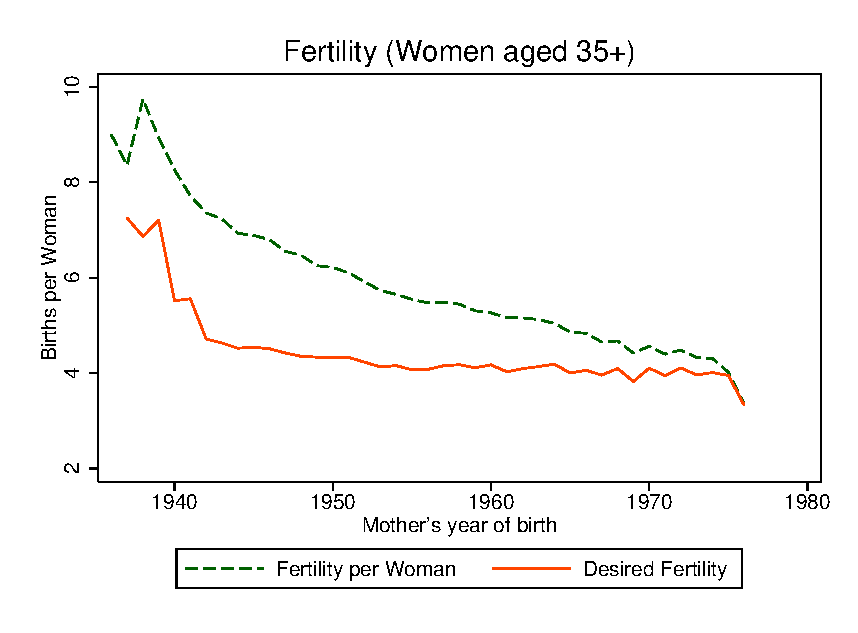
\includegraphics[scale=0.53]{\twinfolder/Figures/ferttrend_35_all.eps}
  \caption{Trends in Fertility}
  \label{TWINfig:fertrend}
\end{subfigure}%
\begin{subfigure}{.5\textwidth}
  \centering
  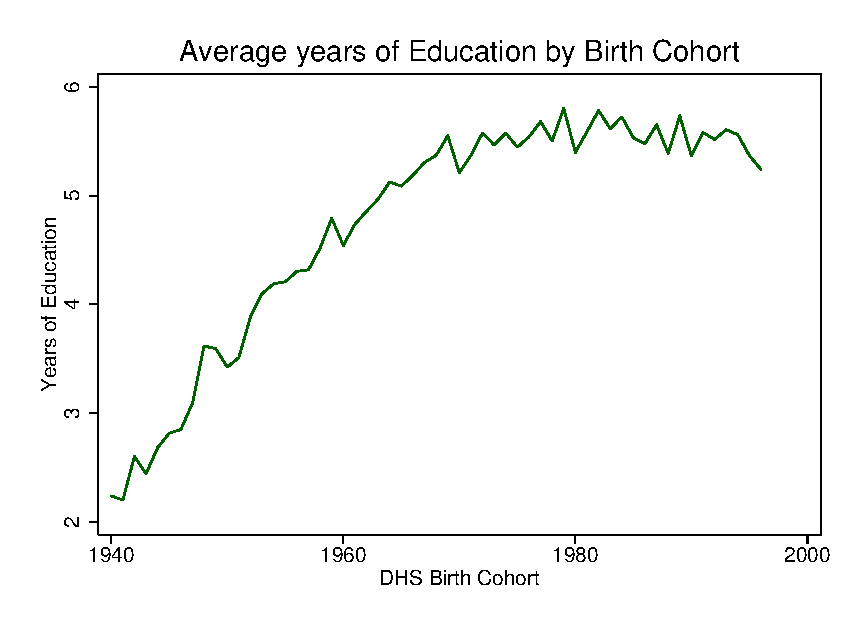
\includegraphics[scale=0.52]{\twinfolder/Figures/eductrend_all.eps}
  \caption{Trend in Education}
  \label{TWINfig:eductrend}
\end{subfigure}
\caption{Education and Fertility}
\label{TWINfig:trends}
\floatfoot{Note to figure \ref{TWINfig:trends}: Cohorts are made up of all individuals 
from the DHS who are over 35 years (for fertility), and over 15 years (for education).  
In each case the sample is restricted to those who have approximately completed fertility 
and education respectively.}
\end{figure}
\vspace{1cm}

\begin{figure}[htpb!]
\begin{center}
\caption{Proportion of Twins of All Births (USA)}
\label{TWINfig:bord}
\includegraphics[scale=0.92]{\twinfolder/Figures/USTwinFLE.eps} 
\end{center}
\end{figure}

\begin{figure}[htpb!]
\begin{center}
\caption{Twin Births and Total Fertility}
\label{TWINfig:births}
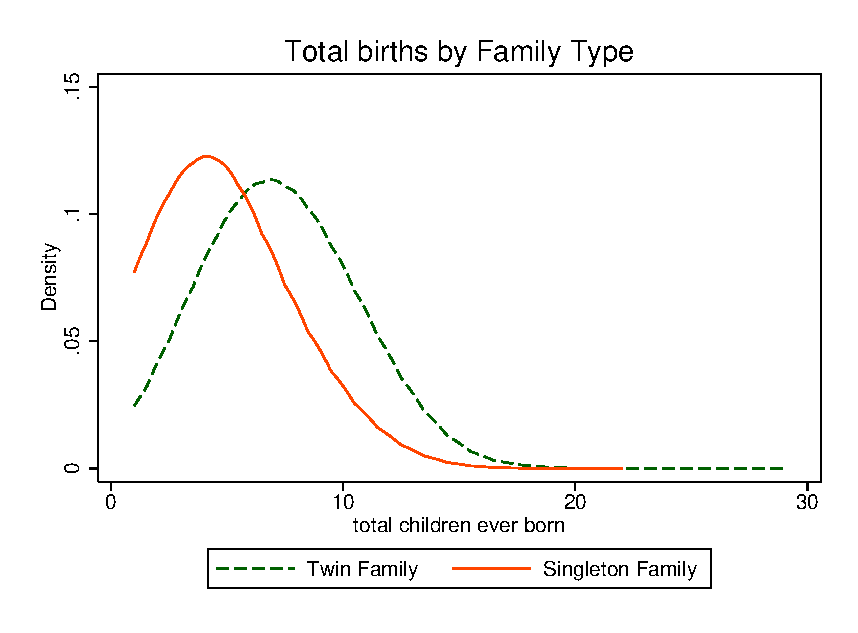
\includegraphics[scale=0.92]{\twinfolder/Figures/famsize.eps} 
\end{center}
\end{figure}

\begin{figure}[htpb!]
\begin{center}
\caption{Proportion of Twins by Birth Order}
\label{TWINfig:bord}
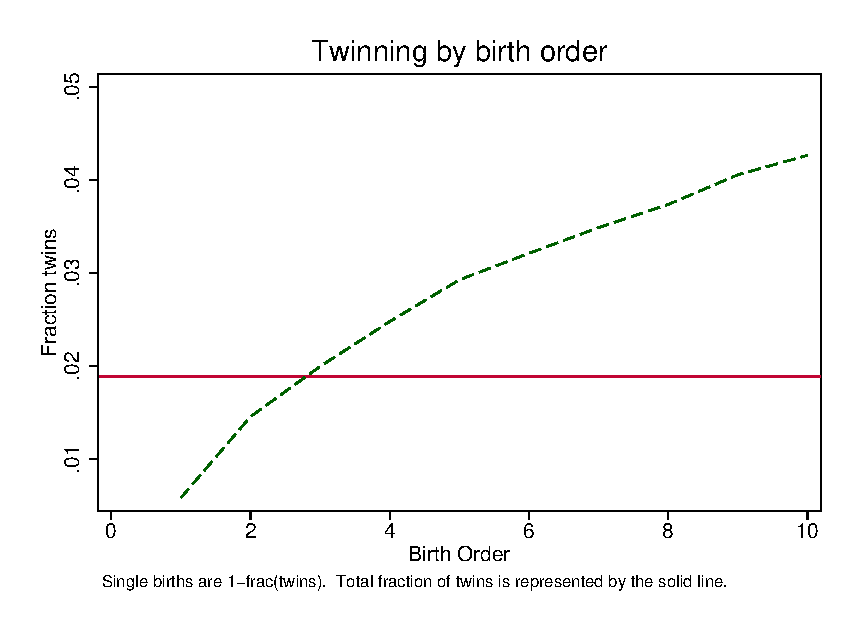
\includegraphics[scale=0.92]{\twinfolder/Figures/twinbybord.eps} 
\end{center}
\end{figure}

\begin{figure}[htpb!]
\begin{center}
\caption{Intra- and Inter-country trends: height and twinning}
\label{TWINfig:arrows}
\includegraphics[scale=0.86]{\twinfolder/Figures/height_country.eps} 
\end{center}
\end{figure}

%\begin{figure}[htpb!]
%\begin{center}
%\caption{Distribution of Ideal Family Size}
%\label{TWINfig:ideal}
%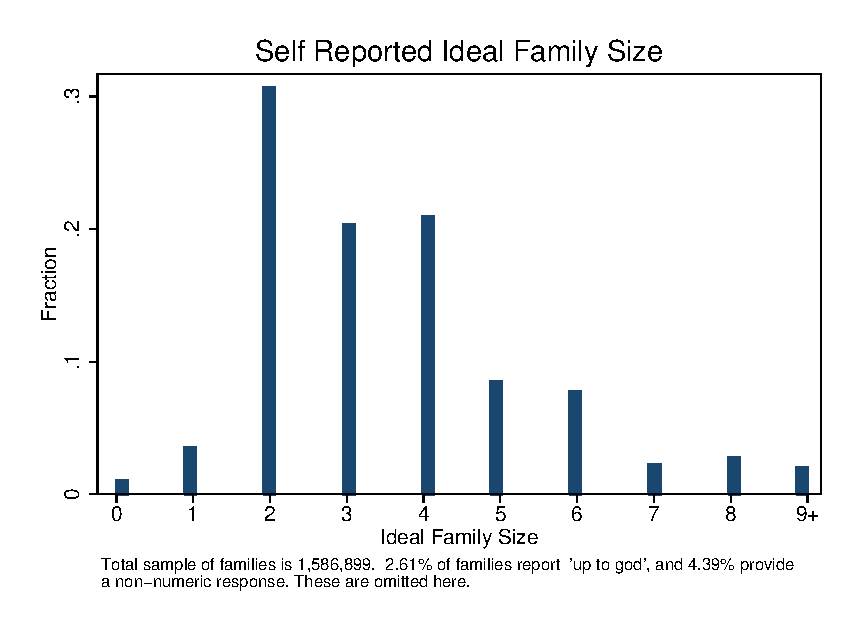
\includegraphics[scale=0.92]{\twinfolder/Figures/idealfamsize.eps} 
%\end{center}
%\end{figure}

%\begin{figure}[htpb!]
%\begin{center}
%\caption{Ideal and Actual Fertility}
%\label{TWINfig:idealactual}
%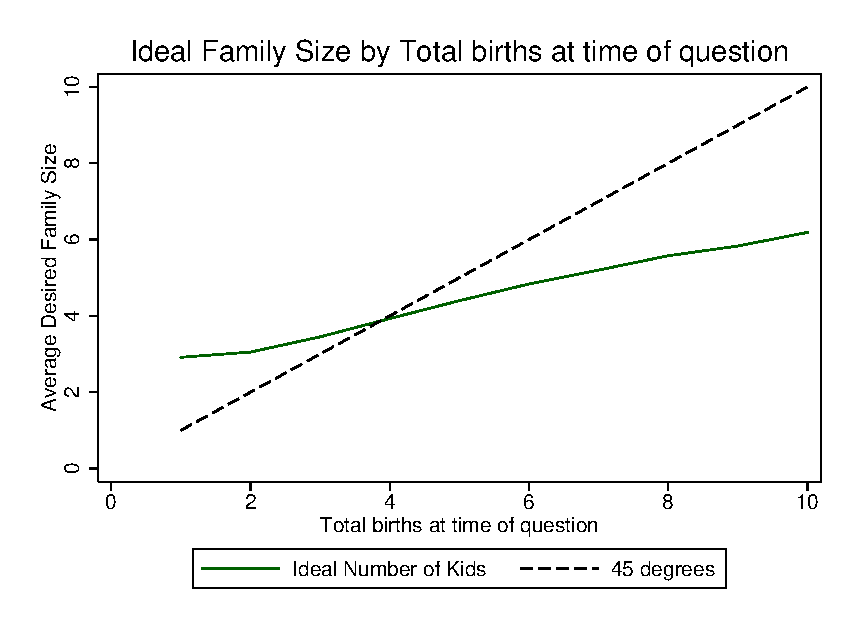
\includegraphics[scale=0.92]{\twinfolder/Figures/idealfam_fert.eps} 
%\end{center}
%\end{figure}

\begin{figure}[htpb!]
\begin{center}
\caption{Relaxing Strict Exogeneity (two plus)}
\label{TWINfig:ltz2}
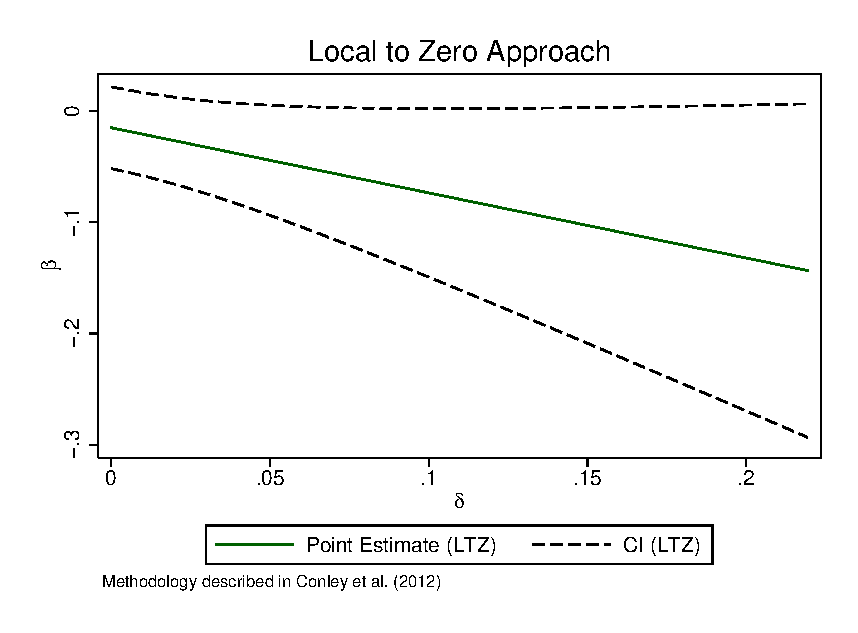
\includegraphics[scale=0.88]{\twinfolder/Figures/LTZ_two.eps}
\vspace{-8mm}
\floatfoot{Note to figure \ref{TWINfig:ltz2}: See note to Figure \ref{TWINfig:ltz3}}
\end{center}
\end{figure}

\begin{figure}[htpb!]
\begin{center}
\caption{Relaxing Strict Exogeneity (three plus)}
\label{TWINfig:ltz3}
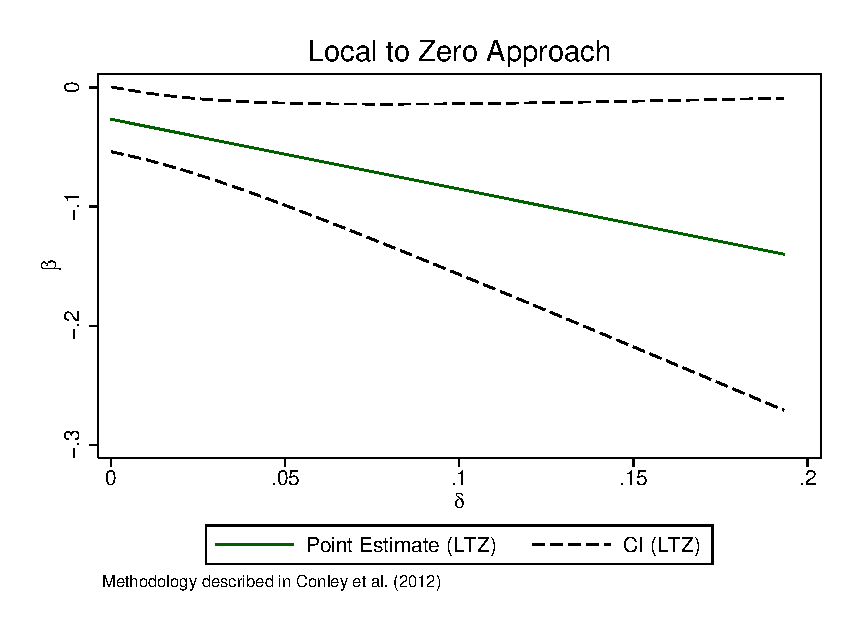
\includegraphics[scale=0.88]{\twinfolder/Figures/LTZ_three.eps} 
\floatfoot{Note to figure \ref{TWINfig:ltz3}: Confidence intervals and point estimates 
are calculated according to \citet{Conleyetal2012}.  Estimates reflect a range of priors 
regarding the validity of the exclusion restriction required to consistently estimate 
$\hat\beta_{fert}$ using twinning in a 2SLS framework.  The local to zero (LTZ) 
approach applied here assumes that $\gamma$, the sign on the instrument when included
in the first stage, is distributed $\gamma\sim U(0,\delta)$.  Further discussion 
is provided in the body of the text and table \ref{TWINtab:Conley}.}
\end{center}
\end{figure}




\newpage
\section*{Tables}
\begin{table}[htpb!]\caption{Summary Statistics} 
\label{TWINtab:sumstats}\begin{center}\scalebox{0.99}{\begin{tabular}{lccccc}
\toprule \toprule 
&\multicolumn{2}{c}{Low Income}&\multicolumn{2}{c}{Middle Income}\\ 
\cmidrule(r){2-3} \cmidrule(r){4-5}
& Single & Twins & Single & Twins & All \\ \midrule 
\textsc{Fertility} & & & & & \\ 
Fertility&3.749&6.223&3.412&5.584&3.689\\
&(2.392)&(2.622)&(2.308)&(2.687)&(2.406)\\
Desired Family Size&4.193&5.328&3.380&4.190&3.921\\
&(2.530)&(2.885)&(2.130)&(2.555)&(2.440)\\
Fraction Twin & \multicolumn{2}{c}{  0.0200}& \multicolumn{2}{c}{  0.0179 } &  0.0191\\
& \multicolumn{2}{c}{(0.1402)}& \multicolumn{2}{c}{(0.1326)} & (0.1370)\\
Birth Order Twin & \multicolumn{2}{c}{   4.664}& \multicolumn{2}{c}{   4.016 }&   4.410\\
& \multicolumn{2}{c}{(2.465)}& \multicolumn{2}{c}{(2.374)}& (2.450)\\
\textsc{Mother's Characteristics}&&&&&\\ Age
&31.22&34.52&32.32&35.61&31.72\\
&(8.238)&(7.381)&(8.356)&(7.428)&(8.293)\\
Education&3.859&3.222&6.690&5.906&4.885\\
&(4.327)&(3.991)&(4.795)&(5.023)&(4.706)\\
Height&155.5&157.6&155.6&157.2&155.6\\
&(7.093)&(7.065)&(6.966)&(6.945)&(7.053)\\
BMI&21.90&22.50&25.90&26.63&23.39\\
&(4.027)&(4.175)&(5.118)&(5.512)&(4.867)\\
Pr(BMI)$<$18.5&0.175&0.125&0.0346&0.0276&0.122\\
&(0.380)&(0.331)&(0.183)&(0.164)&(0.327)\\
Actual Births$>$Desired&0.310&0.526&0.324&0.575&0.321\\
&(0.463)&(0.499)&(0.468)&(0.494)&(0.467)\\
\textsc{Children's Outcomes}&&&&&\\ Education (Years)
&3.660&3.204&5.445&5.043&4.446\\
&(3.576)&(3.293)&(3.867)&(3.760)&(3.810)\\
Education (Z-Score)&-0.00843&-0.0156&0.0119&-0.0428&0.000144\\
&(1.001)&(0.963)&(0.998)&(0.987)&(1.000)\\
No Education (Percent)&0.207&0.222&0.0649&0.0786&0.144\\
&(0.405)&(0.416)&(0.246)&(0.269)&(0.351)\\
Infant Mortality&0.0158&0.0917&0.00946&0.0497&0.0141\\
&(0.125)&(0.289)&(0.0968)&(0.217)&(0.118)\\
Child Mortality&0.0239&0.108&0.0122&0.0535&0.0199\\
&(0.153)&(0.310)&(0.110)&(0.225)&(0.140)\\
\midrule
Number of Countries & 39&39  & 28&28  & 67 \\
Number of Children &2,231,844 &45,654 &1,614,358 &29,430 & 3,921,286 \\
Number of Mothers &875,587 &12,908 &653,969 &8,605 & 1,586,899 \\
\midrule
\multicolumn{6}{p{13.2cm}}{\begin{footnotesize}\textsc{Notes:}  Group means are presented with standard deviation below in parenthesis.  Education is reported as total years attained, and Z-score presents educational attainment relative to country and cohort (mean 0, std deviation 1).  Infant mortality refers to the proportion of children who die before 1 year of age,  while child mortality refers to the proportion who die before 5 years.  Maternal height is reported in cm, and BMI is weight in kg over height in metres squared.  Summary statistics are for the full sample of 1,586,899
 mothers responding to any publicly available DHS survey.  For a full list of country and years of survey, see appendix table \ref{TWINtab:countries}.\end{footnotesize}} \\ \bottomrule \end{tabular}}\end{center}\end{table}


\begin{landscape}\begin{table}[htpb!]\caption{Fertility and the Twin Instrument: Literature} 
\label{TWINtab:Lit}\begin{center}\begin{tabular}{p{4cm}p{5cm}p{5cm}p{2cm}p{1.22cm}p{1.22cm}}
\toprule \toprule 
&&&&\multicolumn{2}{c}{Estimates}\\ \cmidrule(r){5-6}
Author & Data, Period & Controls Included & Sample & \ \ OLS & \ \ IV \\ \midrule 
(1) \citet{Blacketal2005} & 
Norway matched administrative files of
individuals aged 16-74 during 1986-2000,
(children $>$ 25 years). Outcome is 
completed years of education. & 
Age, parents' age, parents' education, 
sex. &  \begin{tabular}[t]{@{}l@{}} Two Plus \\ \\ Three Plus \\ \\ Four Plus \end{tabular}
& -0.060 (0.003) -0.076 (0.004) -0.059 (0.006)
& -0.038 (0.047) -0.016 (0.044) -0.024 (0.059) \\
&&&&& \\
(2) \citet{Caceres2006} & 
USA 1980 Census Five-Percent Public Use Micro Sample.
Children aged 6-16 years. Outcome (reported here) 
is an indicator of whether the child is behind his
or her cohort. & Age, state of residence, mother's
education, race, mother's age, sex. &
\begin{tabular}[t]{@{}l@{}} Two Plus \\ \\ Three Plus \end{tabular}
& 0.011 (0.000) 0.017 (0.001)
& 0.002 (0.003) 0.010 (0.006) \\
&&&&& \\
(3) \citet{Angristetal2010} & 
Israel 20\% public-use microdata samples
from 1995 and 1983 censuses, 18-60 year old respondents.
Outcome (reported here) is highest grade completed. &
Age, missing month of birth, mother's age, age at first birth
and age at immigration, mother's and father's 
place of birth, and census year. &
\begin{tabular}[t]{@{}l@{}} Two Plus \\ \\ Three Plus \end{tabular}
& -0.145 (0.005) -0.143 (0.005)
& 0.174 (0.166) 0.167 (0.117) \\
&&&&& \\
(4) \citet{Lietal2008} &
The 1 percent sample of the 1990 Chinese Population Census.
Subjects are 6-17 year olds with mothers who are 35 years of age or
younger.  Outcome (reported here) is years of schooling. 
& Child age, gender, ethnic group, birth order, and place of residence.
Parental age and educational level.
&
\begin{tabular}[t]{@{}l@{}} Two Plus \\ \\ Three Plus \end{tabular}
& -0.031 (-29.6)\textsuperscript{\dag} -0.038 (-21.4)\textsuperscript{\dag}
& 0.002 (0.18)\textsuperscript{\dag} -0.024 (-1.70)\textsuperscript{\dag} \\
&&&&& \\
(5) \citet{FitzsimonsMalde2014} &
Mexican Survey data (ENCASEH) from 1996-1999.  
Subjects are 12-17 year olds.  Outcome (reported here)
is years of schooling. & Parent's age, parents' years of schooling and
schooling dummies, birth spacing, household goods (rooms, land, water, etc).
&
\begin{tabular}[t]{@{}l@{}} Two Plus \\ \\ Three Plus \\ \\ Four Plus \end{tabular}
& -0.020 (0.001) -0.020 (0.001) -0.018 (0.002)
& -0.019 (0.015) 0.007 (0.025) -0.032 (0.036) \\
&&&&& \\




\end{tabular}\end{center}\end{table}\end{landscape}



\begin{landscape}\begin{table}[htpb!]\begin{center}\begin{tabular}{p{4cm}p{5cm}p{5cm}p{2cm}p{1.3cm}p{1.3cm}}
\midrule
&&&&\multicolumn{2}{c}{Estimates}\\ \cmidrule(r){5-6}
Author & Data, Period & Controls Included & Sample& \ \ OLS &\ \ IV \\ \midrule 
(6) \citet{RosenzweigZhang2009} & 
The Chinese Child Twins Survey (CCTS), 2002-2003.
Individuals selected from twins' (aged 7-18) and
non-twin households. Outcome (reported here) is years of schooling
 & 
Mother's age at time of birth, child gender and age.
 &  \begin{tabular}[t]{@{}l@{}} Reduced Form \\ \\ Reduced Form \\ + Bwt \end{tabular}
& \multicolumn{2}{c}{ 
\begin{tabular}[t]{@{}l@{}} -0.307 \\ (1.92)\textsuperscript{\dag} 
\\ -0.225 \\ (1.31)\textsuperscript{\dag} \end{tabular}} \\
&&&&& \\
(7) \citet{SouzaPonczek2012} & 
1991 Brazilian Census microdata, 10 and 20\% sample.
Children of 10-15 years, and 18-20 years old.  Outcome
reported here is years of school completed.
 & 
Child's gender, age and race controls,; mother and family head's 
years of schooling, and age.
&\begin{tabular}[t]{@{}l@{}} Two Plus \\ (M) \\ Two Plus \\ (F) \\ Three Plus \\ (M) \\ Three Plus \\ (F) \end{tabular}
& -0.233 (0.010) -0.277 (0.015) -0.230 (0.010) -0.283 (0.015)
& -0.137 (0.146) -0.372 (0.198) -0.060 (0.164) -0.634 (0.194) \\
&&&&& \\


\bottomrule 
\multicolumn{6}{p{20cm}}{\begin{footnotesize} Notes: Individual sources discussed further in the body of the text.  Estimates reported in each study are presented along with their standard errors in parenthesis. Parentheses
marked as \textsuperscript{\dag} contain the t-statistic rather than the standard error.\end{footnotesize}} 
\end{tabular}\end{center}\end{table}\end{landscape}



\begin{landscape}\begin{table}[htpb!] 
\caption{Probability of Giving Birth to Twins} \label{TWINtab:twinreg1} 
\begin{center}\begin{tabular}{lcccccc} \toprule \toprule 
&(1)&(2)&(3)&(4)&(5)&(6)\\
Twin$\times$100&All&\multicolumn{2}{c}{Income}&\multicolumn{2}{c}{Time}&Prenatal\\
 \cmidrule(r){3-4} \cmidrule(r){5-6} 
&&Low inc&Middle inc&1990-2013&1972-1989&\\\midrule
\begin{footnotesize}\end{footnotesize}&\begin{footnotesize}\end{footnotesize}&\begin{footnotesize}\end{footnotesize}&\begin{footnotesize}\end{footnotesize}&\begin{footnotesize}\end{footnotesize}&\begin{footnotesize}\end{footnotesize}&\begin{footnotesize}\end{footnotesize}\\
Age&0.491***&0.489***&0.498***&0.587***&0.168***&0.632***\\
&(0.026)&(0.033)&(0.045)&(0.030)&(0.064)&(0.040)\\
Age Squared&-0.006***&-0.006***&-0.007***&-0.008***&-0.000&-0.009***\\
&(0.000)&(0.001)&(0.001)&(0.001)&(0.001)&(0.001)\\
Age First Birth&-0.051***&-0.082***&-0.002&-0.050***&-0.051***&-0.041***\\
&(0.008)&(0.010)&(0.013)&(0.009)&(0.015)&(0.013)\\
Education (years)&0.027*&0.065***&-0.008&0.044**&-0.008&-0.071**\\
&(0.016)&(0.021)&(0.027)&(0.019)&(0.028)&(0.028)\\
Education squared&-0.001&-0.005**&0.001&-0.002&0.002&0.003\\
&(0.001)&(0.002)&(0.002)&(0.001)&(0.002)&(0.002)\\
Height&0.057***&0.056***&0.058***&0.063***&0.038***&0.059***\\
&(0.004)&(0.005)&(0.006)&(0.005)&(0.007)&(0.007)\\
BMI&0.050***&0.059***&0.043***&0.046***&0.056***&0.045***\\
&(0.006)&(0.008)&(0.008)&(0.007)&(0.009)&(0.011)\\
Prenatal (Doctor)&&&&&&0.917***\\
&&&&&&(0.129)\\
Prenatal (Nurse)&&&&&&0.076\\
&&&&&&(0.109)\\
Prenatal (None)&&&&&&-0.479***\\
&&&&&&(0.133)\\
&&&&&&\\R-squared&0.01&0.01&0.01&0.01&0.00&0.01\\
Observations &2271948&1430703&841245&1660253&611695&624990\\
\hline\hline\multicolumn{7}{p{14.3cm}}{\begin{footnotesize}\textsc{Notes:} All specifications include a full set of year of birth and  country dummies, and are estimated as linear probability models.  Twin is multiplied by 100 for presentation.  Height is measured in cm  and BMI is weight in kg divided by height in metres squared. l  Prenatal care variables are only recoreded for recent births.  As  such, column (6) is estimated only for that subset of births where  these observations are made.
$^{*}$p$<$0.1; $^{**}$p$<$0.05; $^{***}$p$<$0.01
 \end{footnotesize}}\\ \hline \normalsize \end{tabular}\end{center}\end{table}\end{landscape} 

\begin{table}[htpb!]
\caption{Test of hypothesis that women who bear twins have better prior health}\label{TWINtab:IMR}\begin{center}\begin{tabular}{lccc}
\toprule \toprule 
\textsc{Infant Mortality (per 100 births)}& Base & +S\&H & Observations \\ \midrule 
\begin{footnotesize}\end{footnotesize}& 
\begin{footnotesize}\end{footnotesize}& 
\begin{footnotesize}\end{footnotesize}& 
\begin{footnotesize}\end{footnotesize}\\ 
Treated (2+)\hspace{5mm}\hspace{5mm}\hspace{5mm}\hspace{5mm}\hspace{5mm}\hspace{5mm}&-2.065***&-2.110***&503785\\
&(0.212)&(0.213)&\\
Treated (3+)\hspace{5mm}&-4.619***&-4.632***&686931\\
&(0.201)&(0.201)&\\
Treated (4+)&-4.257***&-4.243***&676303\\
&(0.183)&(0.183)&\\
Treated (5+)&-3.353***&-3.324***&587919\\
&(0.183)&(0.183)&\\
\midrule\multicolumn{4}{p{12.1cm}}{\begin{footnotesize}\textsc{Notes:} The sample for these regressions consist of all children who have been entirely exposed to the risk of infant mortality (ie those over 1 year of age). Subsamples 2+, 3+, 4+ and 5+ are generated to allow comparison of children born at similar birth orders.  For a full description of these groups see the the body of the paper or notes to table \ref{TWINtab:IVAll}. Treated=1 refers to children who are born before a twin while Treated=0 refers to children of similar birth orders not born before a twin.  Base and S+H controls are described in table \ref{TWINtab:IVAll}.$^{*}$p$<$0.1; $^{**}$p$<$0.05; $^{***}$p$<$0.01 
\end{footnotesize}} \\ \bottomrule 
\end{tabular}\end{center}\end{table}
\begin{table}[htpb]
\caption{Probability of Giving Births to Twins (NHIS, USA)}
\begin{center}
\scalebox{0.64}{
\begin{tabular}{lcc} \toprule
&(1)&(2) \\
VARIABLES&Twin$\times$100&Twin$\times$100 \\ \midrule
&& \\
Mother's Height&0.0416**&0.0406** \\
&(0.0201)&(0.0201) \\
Mother's Education&0.0084&0.0033 \\
&(0.0162)&(0.0164) \\
Smokes (pre-Pregnancy)&-0.119&-0.0983 \\
&(0.115)&(0.116) \\
Mother's Age&0.0121&0.0108 \\
&(0.0446)&(0.0446) \\
Mother's Age$^2$ &-0.0008&-0.0008 \\
&(0.0006)&(0.0006) \\
Age First Birth &0.166***&0.164*** \\
&(0.0135)&(0.0136) \\
BMI &0.0123***&0.0130*** \\
&(0.0034)&(0.0034) \\
Mother Good Health&&0.203* \\
&&(0.116) \\
Mother Poor Health&&-0.00284 \\
&&(0.189) \\
Constant&-4.091***&-4.101*** \\
&(1.542)&(1.543) \\
&& \\
Observations&105,879&105,879 \\
R-squared&0.004&0.004 \\ \midrule
%\multicolumn{3}{ p{5cm} }{\begin{footnotesize}\textsc{Notes:} Standard errors in parentheses. *** p$<$0.01; ** p$<$0.05; * p$<$0.1\end{footnotesize}}\bottomrule
\end{tabular}}
\end{center}
\end{table}



\input{\twinfolder/Tables/Alderman.tex}
\input{\twinfolder/Tables/NepalRegs2.tex}

\begin{landscape}\begin{table}[!htbp] \centering 
\caption{OLS Estimates of the Q-Q Trade-off} 
 \vspace{4mm}\label{TWINtab:OLS} 
\begin{tabular}{lcccccc} \toprule \toprule 
&Base&+&+&Desired&Altonji&Altonji\\
&Controls&Socioec&Health&&Ratio 1&Ratio 2\\\midrule
\textsc{Panel A: All Countries}&&&&&&\\
Fertility &-0.115***&-0.0777***&-0.0751***&-0.0717***&2.083&1.882\\
&(0.000815)&(0.000776)&(0.000771)&(0.000838)&&\\
Fertility$\times$desire&&&&-0.00558***&&\\
&&&&(0.000495)&&\\
&&&&&&\\
Observations &1,334,874&1,334,874&1,334,874&1,334,874&&\\
R$^2$&0.094&0.161&0.167&0.168&&\\\midrule
\textsc{Panel B: Low Income}&&&&&&\\
Fertility &-0.110***&-0.0734***&-0.0712***&-0.0668***&2.005&1.835\\
&(0.00106)&(0.000988)&(0.000975)&(0.00107)&&\\
Fertility$\times$desire&&&&-0.00674***&&\\
&&&&(0.000608)&&\\
&&&&&&\\
Observations &831,476&831,476&831,476&831,476&&\\
R$^2$&0.091&0.171&0.181&0.182&&\\\midrule
\textsc{Panel C: Middle Income}&&&&&&\\
Fertility &-0.125***&-0.0875***&-0.0854***&-0.0839***&2.333&2.157\\
&(0.00128)&(0.00126)&(0.00126)&(0.00134)&&\\
Fertility$\times$desire&&&&-0.00266***&&\\
&&&&(0.000846)&&\\
&&&&&&\\
Observations &503,398&503,398&503,398&503,398&&\\
R$^2$&0.106&0.154&0.156&0.156&&\\\hline\hline
\multicolumn{7}{p{15.8cm}}{\begin{footnotesize}\textsc{Notes:} Base controls consist of child gender, mother's age and age squared mother's age at first birth, child age, country, and year of birth dummies.  Socioeconomic augments `Base' to include mother's education and education squared, and Health includes mother's height and BMI. ``Desire'' takes 1 if the child is born before the family reaches it's desired size, and 0 if the child is born after the desired size is reached. The \citet{Altonjietal2005} ratio determines how important unobservable factors must be compared with included observables to imply that the true effect of fertilty on educational attainment is equal to zero.  Ratio 1 compares no controls to socioeconomic controls, while ratio 2 compares no controls to socioeconomic and health controls. Standard errors are clustered at the level of the mother.
$^{*}$p$<$0.1; $^{**}$p$<$0.05; $^{***}$p$<$0.01\end{footnotesize}}\\  
\bottomrule \normalsize\end{tabular}\end{table}\end{landscape} 

\begin{table}[htpb!]\caption{Principal IV Results}
\label{TWINtab:IVAll}
\begin{center}\scalebox{0.55}{
\begin{tabular}{lcccp{2mm}cccp{2mm}ccc}
\toprule \toprule 
&\multicolumn{3}{c}{2+}&&\multicolumn{3}{c}{3+}&&\multicolumn{3}{c}{4+}\\ \cmidrule(r){2-4} \cmidrule(r){6-8} \cmidrule(r){10-12} 
\textsc{School Z-Score}&Base&+H&+S\&H&&Base&+H&+S\&H&&Base&+H&+S\&H\\ \midrule 
\begin{footnotesize}\end{footnotesize}& 
\begin{footnotesize}\end{footnotesize}& 
\begin{footnotesize}\end{footnotesize}& 
\begin{footnotesize}\end{footnotesize}& 
\begin{footnotesize}\end{footnotesize}& 
\begin{footnotesize}\end{footnotesize}& 
\begin{footnotesize}\end{footnotesize}& 
\begin{footnotesize}\end{footnotesize}& 
\begin{footnotesize}\end{footnotesize}& 
\begin{footnotesize}\end{footnotesize}& 
\begin{footnotesize}\end{footnotesize}& 
\begin{footnotesize}\end{footnotesize}\\ 
\multicolumn{12}{l}{\textbf{All}}\\ 
Fertility&0.006&-0.026&-0.026&&-0.004&-0.036&-0.038*&&-0.017&-0.036&-0.035*\\
&(0.029)&(0.027)&(0.026)&&(0.024)&(0.022)&(0.021)&&(0.025)&(0.023)&(0.021)\\
\begin{footnotesize}\end{footnotesize}&\begin{footnotesize}\end{footnotesize}&\begin{footnotesize}\end{footnotesize}&\begin{footnotesize}\end{footnotesize}&\begin{footnotesize}\end{footnotesize}&\begin{footnotesize}\end{footnotesize}&\begin{footnotesize}\end{footnotesize}&\begin{footnotesize}\end{footnotesize}&\begin{footnotesize}\end{footnotesize}&\begin{footnotesize}\end{footnotesize}&\begin{footnotesize}\end{footnotesize}&\begin{footnotesize}\end{footnotesize}\\Observations&249536&249536&249536&&375987&375987&375987&&385389&385389&385389\\
\multicolumn{12}{l}{\textbf{Low-Income}}\\ 
Fertility&0.035&0.008&0.012&&0.016&-0.016&-0.027&&-0.011&-0.031&-0.024\\
&(0.034)&(0.032)&(0.031)&&(0.030)&(0.028)&(0.026)&&(0.029)&(0.027)&(0.025)\\
\begin{footnotesize}\end{footnotesize}&\begin{footnotesize}\end{footnotesize}&\begin{footnotesize}\end{footnotesize}&\begin{footnotesize}\end{footnotesize}&\begin{footnotesize}\end{footnotesize}&\begin{footnotesize}\end{footnotesize}&\begin{footnotesize}\end{footnotesize}&\begin{footnotesize}\end{footnotesize}&\begin{footnotesize}\end{footnotesize}&\begin{footnotesize}\end{footnotesize}\\Observations&149602&149602&149602&&232371&232371&232371&&246622&246622&246622\\
\multicolumn{12}{l}{\textbf{Middle-Income}}\\ 
Fertility&-0.065&-0.087*&-0.093**&&-0.046&-0.079**&-0.067*&&-0.027&-0.048&-0.054\\
&(0.053)&(0.049)&(0.047)&&(0.040)&(0.036)&(0.035)&&(0.043)&(0.040)&(0.037)\\
\begin{footnotesize}\end{footnotesize}&\begin{footnotesize}\end{footnotesize}&\begin{footnotesize}\end{footnotesize}&\begin{footnotesize}\end{footnotesize}&\begin{footnotesize}\end{footnotesize}&\begin{footnotesize}\end{footnotesize}&\begin{footnotesize}\end{footnotesize}&\begin{footnotesize}\end{footnotesize}&\begin{footnotesize}\end{footnotesize}&\begin{footnotesize}\end{footnotesize}\\Observations&99934&99934&99934&&143616&143616&143616&&138767&138767&138767\\
\multicolumn{12}{l}{\textbf{Adjusted Fertility}}\\ 
Fertility&0.017&-0.052&-0.055&&-0.013&-0.073*&-0.077*&&-0.033&-0.068&-0.066*\\
&(0.065)&(0.056)&(0.054)&&(0.047)&(0.043)&(0.040)&&(0.045)&(0.042)&(0.039)\\
\begin{footnotesize}\end{footnotesize}&\begin{footnotesize}\end{footnotesize}&\begin{footnotesize}\end{footnotesize}&\begin{footnotesize}\end{footnotesize}&\begin{footnotesize}\end{footnotesize}&\begin{footnotesize}\end{footnotesize}&\begin{footnotesize}\end{footnotesize}&\begin{footnotesize}\end{footnotesize}&\begin{footnotesize}\end{footnotesize}&\begin{footnotesize}\end{footnotesize}\\Observations&249505&249505&249505&&375957&375957&375957&&385363&385363&385363\\
\multicolumn{12}{l}{\textbf{Twins and Pre-Twins}}\\ 
Fertility&-0.021&-0.073***&-0.078***&&-0.019&-0.062***&-0.067***&&-0.018&-0.039**&-0.046**\\
&(0.024)&(0.021)&(0.020)&&(0.020)&(0.018)&(0.018)&&(0.021)&(0.019)&(0.018)\\
\begin{footnotesize}\end{footnotesize}&\begin{footnotesize}\end{footnotesize}&\begin{footnotesize}\end{footnotesize}&\begin{footnotesize}\end{footnotesize}&\begin{footnotesize}\end{footnotesize}&\begin{footnotesize}\end{footnotesize}&\begin{footnotesize}\end{footnotesize}&\begin{footnotesize}\end{footnotesize}&\begin{footnotesize}\end{footnotesize}&\begin{footnotesize}\end{footnotesize}\\Observations&488815&488815&488815&&563177&563177&563177&&523197&523197&523197\\
\bottomrule
\end{tabular}}\end{center}\end{table}

\begin{table}[htpb!]\caption{NHIS Estimates (USA): Education and Health}
\label{TWINtab:NHISAll}
\begin{center}
\scalebox{0.52}{
\begin{tabular}{lcccp{2mm}cccp{2mm}ccc}
\toprule \toprule 
&\multicolumn{3}{c}{2+}&&\multicolumn{3}{c}{3+}&&\multicolumn{3}{c}{4+}\\ \cmidrule(r){2-4} \cmidrule(r){6-8} \cmidrule(r){10-12} 
&Base&+H&+S\&H&&Base&+H&+S\&H&&Base&+H&+S\&H\\ \midrule 
\begin{footnotesize}\end{footnotesize}& 
\begin{footnotesize}\end{footnotesize}& 
\begin{footnotesize}\end{footnotesize}& 
\begin{footnotesize}\end{footnotesize}& 
\begin{footnotesize}\end{footnotesize}& 
\begin{footnotesize}\end{footnotesize}& 
\begin{footnotesize}\end{footnotesize}& 
\begin{footnotesize}\end{footnotesize}& 
\begin{footnotesize}\end{footnotesize}& 
\begin{footnotesize}\end{footnotesize}& 
\begin{footnotesize}\end{footnotesize}& 
\begin{footnotesize}\end{footnotesize}\\ 
\multicolumn{12}{l}{\textbf{OLS}}\\ 
School Z-Score&-0.043***&-0.033***&-0.027***&&-0.036***&-0.028***&-0.020**&&-0.010&-0.004&0.002\\
&(0.005)&(0.006)&(0.006)&&(0.008)&(0.009)&(0.009)&&(0.018)&(0.018)&(0.018)-\\
Excellent Health&-0.012***&-0.005***&-0.004*&&-0.018***&-0.010***&-0.008***&&-0.028***&-0.019***&-0.017***\\
&(0.002)&(0.002)&(0.002)&&(0.004)&(0.003)&(0.003)&&(0.006)&(0.005)&(0.005)\\

\begin{footnotesize}\end{footnotesize}&\begin{footnotesize}\end{footnotesize}&\begin{footnotesize}\end{footnotesize}&\begin{footnotesize}\end{footnotesize}&\begin{footnotesize}\end{footnotesize}&\begin{footnotesize}\end{footnotesize}&\begin{footnotesize}\end{footnotesize}&\begin{footnotesize}\end{footnotesize}&\begin{footnotesize}\end{footnotesize}&\begin{footnotesize}\end{footnotesize}&\begin{footnotesize}\end{footnotesize}&\begin{footnotesize}\end{footnotesize}\\
\multicolumn{12}{l}{\textbf{IV}}\\ 
School Z-Score&-0.064&-0.074&-0.077&&-0.027&-0.037&-0.036&&-0.094&-0.099&-0.113\\
&(0.063)&(0.059)&(0.058)&&(0.065)&(0.064)&(0.065)&&(0.152)&(0.155)&(0.150)\\

Excellent Health&0.013&0.022&0.019&&-0.016&-0.054*&-0.055*&&0.057&0.017&0.006\\
&(0.025)&(0.020)&(0.020)&&(0.038)&(0.031)&(0.031)&&(0.058)&(0.054)&(0.052)\\
\begin{footnotesize}\end{footnotesize}&\begin{footnotesize}\end{footnotesize}&\begin{footnotesize}\end{footnotesize}&\begin{footnotesize}\end{footnotesize}&\begin{footnotesize}\end{footnotesize}&\begin{footnotesize}\end{footnotesize}&\begin{footnotesize}\end{footnotesize}&\begin{footnotesize}\end{footnotesize}&\begin{footnotesize}\end{footnotesize}&\begin{footnotesize}\end{footnotesize}&\begin{footnotesize}\end{footnotesize}&\begin{footnotesize}\end{footnotesize}\\
\multicolumn{12}{l}{\textbf{Descriptives}}\\ 
School Z-Score&-0.0233&&&&-0.0363&&&&-0.0628&&\\
&(0.993)&&&&(1.041)&&&&(1.086)&&\\
Excellent Health&0.533&&&&0.511&&&&0.490&&\\
&(0.499)&&&&(0.500)&&&&(0.500)&&\\
\begin{footnotesize}\end{footnotesize}&\begin{footnotesize}\end{footnotesize}&\begin{footnotesize}\end{footnotesize}&\begin{footnotesize}\end{footnotesize}&\begin{footnotesize}\end{footnotesize}&\begin{footnotesize}\end{footnotesize}&\begin{footnotesize}\end{footnotesize}&\begin{footnotesize}\end{footnotesize}&\begin{footnotesize}\end{footnotesize}&\begin{footnotesize}\end{footnotesize}&\begin{footnotesize}\end{footnotesize}&\begin{footnotesize}\end{footnotesize}\\ 
Observations & 75,902 &	75,902 &	75,902 &&	57,413 &	57,413 &	57,413 &&	26,128 &	26,128 &	26,128 \\
Joint F-test Educ &&164.5&64.7&&&101.3&39.6&&&38.0&7.7\\
Joint F-test Health &&34469.6&163.9&&&15335.6&28.4&&&5276.4&17.1\\
\midrule\multicolumn{12}{p{20.6cm}}{\begin{footnotesize}\textsc{Notes:}  
Each cell presents the coefficient of interest from a regression using NHIS survey data (2002-2014). Base controls include child age FE (in months), mother's age, and mother's age at first birth 
plus race dummies for child and mother.  First stage omitted for clarity (generally all around 0.7).  Standard errors are clustered by mother.$^{*}$p$<$0.1; $^{**}$p$<$0.05; $^{***}$p$<$0.01. 
\end{footnotesize}} \\ \bottomrule 
\end{tabular}}\end{center}\end{table}


\begin{table}[htpb!]\caption{`Plausibly Exogenous' Bounds} 
\label{TWINtab:Conley}\begin{center}\begin{tabular}{lcccc}
\toprule \toprule 
&\multicolumn{2}{c}{UCI: $\gamma\in [0,\delta]$}&\multicolumn{2}{c}{LTZ: $\gamma \sim U(0,\delta)$}\\ 
\cmidrule(r){2-3} \cmidrule(r){4-5}
&Lower Bound&Upper Bound&Lower Bound&Upper Bound\\
Two Plus&-0.1860&0.0195&-0.1613&0.0011\\
Three Plus&-0.1710&0.0025&-0.1528&-0.0116\\
Four Plus&-0.1539&-0.0067&-0.1391&-0.0194\\
Five Plus&-0.1373&0.0277&-0.1215&0.0143\\
\midrule\multicolumn{5}{p{11.6cm}}{\begin{footnotesize}\textsc{Notes:} This table presents upper and lower bounds of a 95\% confidence interval for the effects of family size on (standardised) children's education attainment. These are estimated by the methodology of \citet{Conleyetal2012}  under various priors about the direct effect that being from a twin family has on educational outcomes ($\gamma$). In the UCI (union of confidence interval) approach, it is assumed the true $\gamma\in[0,\delta]$, while in the LTZ (local to zero) approach it is assumed that $\gamma\sim U(0,\delta)$.  In each case $\delta$ is estimated by including twinning in the first stage  equation and observing the effect size $\hat\gamma$.  Estimated $\hat\gamma$'s are (respectively for two plus to five plus):   0.1088, 0.0983, 0.0826, 0.0929.\end{footnotesize}}  
\\ \bottomrule \end{tabular}\end{center}\end{table} 




\newpage
\section*{Appendices}
\appendix
\section{IV Estimation of the Quality-Quantity Tradeoff}
\label{scn:IV}
Discuss 2+, 3+, 4+ groups.

\section{Appendix Tables}
\label{scn:appendixtables}

\begin{table}[htpb!]
\caption{Full Survey Countries and Years}
\label{tab:countries}
\begin{center}
\includegraphics[scale=0.75]{./tables/surveycountry1.png} 
\end{center}
\end{table}

\begin{center}
\includegraphics[scale=0.75]{./tables/surveycountry2.png} 
\end{center}

\begin{table}[htpb!]
\caption{Probability of Giving Birth to Multiple Children (ELPI)}
\label{tab:twinreg2}
\begin{center}
\includegraphics[scale=0.9]{./tables/twinreg2.png} 
\end{center}
\end{table}

\begin{table}[htpb!]
\caption{Estimates of the Q-Q Tradeoff using Twin Births (Alternate Outcomes)}
\label{tab:QQAllApp}
\begin{center}
\includegraphics[scale=0.7]{./tables/QQ_All_app.png} 
\end{center}
\end{table}

\begin{table}[htpb!]
\caption{Estimates of the Q-Q Tradeoff using Twin Births -- Pre-twins only}
\label{tab:QQPretwinApp}
\begin{center}
\includegraphics[scale=0.8]{./tables/QQ_Pretwin_app.png} 
\end{center}
\end{table}

\begin{table}[htpb!]
\caption{QQ Tradeoff by Subgroup (Alternate Outcomes)}
\label{tab:Heterog}
\begin{center}
\includegraphics[scale=1]{./tables/Heterog_App.png} 
\end{center}
\end{table}

\begin{landscape}
\begin{table}[htpb!]
\caption{QQ Tradeoff by IV}
\label{tab:Heterog}
\begin{center}
\includegraphics[scale=0.8]{./tables/QQ_IV.png} 
\end{center}
\end{table}
\end{landscape}




\end{spacing}
\end{document}










































































































\subsection{Assessing the Role of Unobservable Determinants of Twin Births}
\label{scn:selection}
Sections \ref{scn:MCS} and \ref{scn:EE} demonstrate that the incidence of omitted twin predictor variables will invalidate the instrumental variable identification strategy.  
Monte Carlo simulations suggest that even a relatively minor correlation between these unobserved terms and the stochastic component of the Q-Q equation can result in estimators 
which perform quantitatively worse than traditional OLS estimators.  However, if we are able to collect data on these variables which influence twin-selection,\footnote{We refer to twin ``selection" 
here not because families choose whether or not to have twins, but rather because certain characteristics make it appear as if families are more likely to select in to multiple 
births.  Once again, a parallel may be drawn with the use of twins as an instrument in situations where IVF treatment is available; in this case it seems less farfetched to speak 
of ``selection'' of multiple births.  The usefulness of this term will become apparent in the analysis which follows (for the OLS analysis), which draws from prior literature on 
selection on observables versus selection on unobservables.} a 2SLS methodology can still be used consistently by including these predictors as controls in the first and second 
stage.  This is a technique employed in previous literature which has included controls for parity, race and mother's age, along with (more recently) mother's education.  The 
credibility of this strategy however relies on the ability to perfectly observe determinant factors which increase the propensity of twin birth.  If we believe that models such 
as (\ref{eqn:twinpred}) are structural representations of twin birth, we can simply include all relevant predictors, and recover consistent estimates of family size.












In what follows, exogenous variables in equation \ref{eqn:2SLSa} will be denoted 
$\mathbf{x_2}$, the endogenous variable $Fert_j$ as $x_1$, the instrumental variable twin as $z_1$, and the outcome variable $Q_{ij}$ as $y$.  
Then, the regressors from equation \ref{eqn:2SLSa} are represented as $\vect{x}=[x_1\ \vect{x}_2']'$ and the instruments from \ref{eqn:2SLSb} as 
$\vect{z}=[z_1\ \vect{x}_2']'$.

In order to derive the asymptotic properties of the estimators of $\vect{\beta}$, we start from the typical instrumental variables estimator
$\vect{\hat{\beta}}_{IV}=(\vect{Z}'\vect{X})^{-1}\vect{Z}'\vect{y} $ where $\vect{Z}$ and $\vect{X}$ are $N \times k$ matrices with $i$\textsuperscript{th} 
row $\vect{z}_i'$ and $\vect{x}_i'$ respectively.  Determining consistency proceeds via the susbstitution of the structural equation for $\vect{y}$:
\vspace{-5mm}
\begin{eqnarray}
\label{eqn:IVderive}
\vect{\hat{\beta}}_{IV}&=&(\vect{Z}'\vect{X})^{-1}\vect{Z}'[\vect{X\beta}+\vect{u}] \nonumber\\
&=&\vect{\beta}+(\vect{Z}'\vect{X})^{-1}\vect{Z}'\vect{u}\nonumber\\
&=&\vect{\beta}+(N^{-1}\vect{Z}'\vect{X})^{-1}N^{-1}\vect{Z}'\vect{u}
\end{eqnarray}
where the final line is included in order to demonstrate consistency via the use of the law of large numbers\footnote{This relies
on the fact that $N^{-1}\vect{Z}'\vect{X}=N^{-1}\sum_i\vect{z}_i\vect{x}_i'$ and likewise for $N^{-1}\vect{Z}'\vect{u}$.  A
complete exposition can be found in Cameron and Trivedi (2006).}.  Consistency of the IV estimator requires that
\begin{eqnarray}
\mathrm{plim} N^{-1}\vect{Z'u}&=&0, \hspace{5mm}\mathrm{and} \label{eqn:IVconsist3}\\ 
\mathrm{plim} N^{-1}\vect{Z'X}&\neq&0, \label{eqn:IVrelevance}
\end{eqnarray}
the typical IV assumptions of consistency (\ref{eqn:IVconsist3}) and relevance (\ref{eqn:IVrelevance}).  

This paper is concerned with the potential endogeneity of twin births.  Where twin births are endogenous, responding to characteristics such as mother's 
health and education and family income, omitting these factors in the structural equation \ref{eqn:2SLSa} will lead to biased and inconsistent estimates of 
$\vect{\hat{\beta}}_{IV}$.  Suppose that relevant (observed or unobserved) factors are omitted from (\ref{eqn:2SLSa}) and (\ref{eqn:2SLSb}) thus being 
relegated to the error terms $u_{ij}$ and $v_{ij}$.  If these omitted variables are correlated with twin birth ($Twin$), this will invalidate the IV strategy via 
the violation of condition (\ref{eqn:IVconsist3}).  This inconsistency follows directly from a rearrangement of (\ref{eqn:IVderive}):
\begin{equation}
\label{eqn:inconsistency}
\vect{\hat{\beta}}_{IV}-\beta=(N^{-1}\vect{Z}'\vect{X})^{-1}N^{-1}\vect{Z}'\vect{u}.
\end{equation}
If twin birth is indeed endogenous and its determinants are omitted from our IV estimation strategy, the magnitude of the inconsistency in 
(\ref{eqn:inconsistency}) will depend upon two things.  Firstly, (inversely) upon the correlation between the exogenous instrumental
variables and the explanatory variables $\vect{x}$, and secondly upon the correlation between the exogenous instrumental component
$\vect{z}$ and u.  We will turn to these points in section \ref{scn:results}.






We provide results from IV estimations of the Q-Q model when including a more comprehensive set of controls than previous papers, fundamentally extending the vector to include 
maternal health variables. This methodology suggests that any effect of family fertility on a child's schooling is insignificant, \emph{if} twin births are exogenous conditional on 
the extended control set.  Monte Carlo simulation suggests however that even a small correlation between twin births and the residual in the Q-Q regression will lead to a 
quantitatively important bias in this estimate.  In order to examine the plausibility that any trade-off exists, recent work by Altonji et al.\ has beed applied to the Q-Q model, suggesting 
that un-observed factors must be more than twice as important as observables in this model to explain away the entire effect of family size on child `quality'.  Particularly in 
low-income countries, this suggests that the plausibility that larger sibship reduces investment per child may be higher than IV estimates suggest.

These results suggest that the Q-Q trade-off may be a relevant phenomenon, however that this trade-off becomes weaker as country incomes rise.  Such a result is consistent 
with a situation in which there are decreasing marginal returns to investments in child quality.  An increase in income which shifts outward the household budget constraint makes 
more of both child quantity and quality feasible. While shifts towards quality at low levels of child investment result in a measured improvement in observable human capital 
outcomes, diminishing returns imply that subsequent fertility reductions yield smaller increases in quality.  This seems to be reflected in the wider literature, with a lack of evidence 
in favour of the Q-Q trade-off in human capital existing in the developed world (Angrist et al., 2010; Black et al., 2005), whereas recent empirical results from developing countries 
provide some supporting evidence (Sanhueza, 2009; Li et al., 2008).  These results have implications for fertility policies in low-income countries.  If policy makers view fertility 
as `too high' due to the burden it places on household finances and the dilution of resources destined to each child, an exogenous shock to family size (such as that imposed 
by maximum fertility rules) should result in an increase in child attainment.  This paper calls into question the validity of such policies in all but the lowest income country groups,
where households appear to face a particularly steep Q-Q trade-off.








\begin{sidewaystable}[!htbp]																					
\caption{Q-Q specification with years of schooling as quality}																					
\vspace{-3mm}																					
\label{tab:YrsEducAPP1}																					
\begin{center}																					
\begin{tabular}{lcccccccccc} \toprule																					
& \multicolumn{5}{c}{2 +} & \multicolumn{5}{c}{5 +} \\ \cmidrule(r){2-6} \cmidrule(r){7-11}																					
& OLS  & OLS & IV & IV  & IV  & OLS  & OLS & IV  & IV  & IV \\ 																					
& No control & All & No control &  Socioec. & + Health & No control & All & No control &  Socioec. & + Health \\ \midrule
\begin{footnotesize}\end{footnotesize}&\begin{footnotesize}\end{footnotesize}&\begin{footnotesize}\end{footnotesize}&\begin{footnotesize}\end{footnotesize}&\begin{footnotesize}\end{footnotesize}&\begin{footnotesize}\end{footnotesize}&\begin{footnotesize}\end{footnotesize}&\begin{footnotesize}\end{footnotesize}&\begin{footnotesize}\end{footnotesize}&\begin{footnotesize}\end{footnotesize}&\begin{footnotesize}\end{footnotesize}\\																					
fertility	&	-0.588**	&	-0.309**	&	0.915	&	0.260	&	0.118	&	-0.492**	&	-0.298**	&	0.0254	&	-0.149	&	-0.246	\\
\vspace{4pt} & \begin{footnotesize}		(0.00962)	\end{footnotesize} & \begin{footnotesize}	(0.00914)	\end{footnotesize} & \begin{footnotesize}	(0.776)	\end{footnotesize} & \begin{footnotesize}	(0.482)	\end{footnotesize} & \begin{footnotesize}	(0.449)	\end{footnotesize} & \begin{footnotesize}	(0.00857)	\end{footnotesize} & \begin{footnotesize}	(0.00810)	\end{footnotesize} & \begin{footnotesize}	(0.286)	\end{footnotesize} & \begin{footnotesize}	(0.247)	\end{footnotesize} & \begin{footnotesize}	(0.238)	\end{footnotesize} \\
mother educ 0	&		&	-4.337**	&		&	-5.585**	&	-5.052**	&		&	-3.344**	&		&	-4.753**	&	-4.353**	\\
\vspace{4pt} & \begin{footnotesize}			\end{footnotesize} & \begin{footnotesize}	(0.0641)	\end{footnotesize} & \begin{footnotesize}		\end{footnotesize} & \begin{footnotesize}	(0.851)	\end{footnotesize} & \begin{footnotesize}	(0.754)	\end{footnotesize} & \begin{footnotesize}		\end{footnotesize} & \begin{footnotesize}	(0.0511)	\end{footnotesize} & \begin{footnotesize}		\end{footnotesize} & \begin{footnotesize}	(0.309)	\end{footnotesize} & \begin{footnotesize}	(0.282)	\end{footnotesize} \\
mother educ 1--4	&		&	-2.874**	&		&	-3.892**	&	-3.488**	&		&	-1.955**	&		&	-3.245**	&	-2.953**	\\
\vspace{4pt} & \begin{footnotesize}			\end{footnotesize} & \begin{footnotesize}	(0.0682)	\end{footnotesize} & \begin{footnotesize}		\end{footnotesize} & \begin{footnotesize}	(0.725)	\end{footnotesize} & \begin{footnotesize}	(0.649)	\end{footnotesize} & \begin{footnotesize}		\end{footnotesize} & \begin{footnotesize}	(0.0546)	\end{footnotesize} & \begin{footnotesize}		\end{footnotesize} & \begin{footnotesize}	(0.251)	\end{footnotesize} & \begin{footnotesize}	(0.231)	\end{footnotesize} \\
mother educ 5--6	&		&	-1.650**	&		&	-2.264**	&	-2.036**	&		&	-0.847**	&		&	-2.003**	&	-1.828**	\\
\vspace{4pt} & \begin{footnotesize}			\end{footnotesize} & \begin{footnotesize}	(0.0665)	\end{footnotesize} & \begin{footnotesize}		\end{footnotesize} & \begin{footnotesize}	(0.455)	\end{footnotesize} & \begin{footnotesize}	(0.411)	\end{footnotesize} & \begin{footnotesize}		\end{footnotesize} & \begin{footnotesize}	(0.0576)	\end{footnotesize} & \begin{footnotesize}		\end{footnotesize} & \begin{footnotesize}	(0.174)	\end{footnotesize} & \begin{footnotesize}	(0.162)	\end{footnotesize} \\
mother educ 7--10	&		&	-0.871**	&		&	-1.229**	&	-1.121**	&		&		&		&	-1.045**	&	-0.971**	\\
\vspace{4pt} & \begin{footnotesize}			\end{footnotesize} & \begin{footnotesize}	(0.0631)	\end{footnotesize} & \begin{footnotesize}		\end{footnotesize} & \begin{footnotesize}	(0.294)	\end{footnotesize} & \begin{footnotesize}	(0.271)	\end{footnotesize} & \begin{footnotesize}		\end{footnotesize} & \begin{footnotesize}		\end{footnotesize} & \begin{footnotesize}		\end{footnotesize} & \begin{footnotesize}	(0.131)	\end{footnotesize} & \begin{footnotesize}	(0.126)	\end{footnotesize} \\
Poor	&		&	-1.937**	&		&	-2.521**	&	-2.243**	&		&	-1.815**	&		&	-2.064**	&	-1.847**	\\
\vspace{4pt} & \begin{footnotesize}			\end{footnotesize} & \begin{footnotesize}	(0.0691)	\end{footnotesize} & \begin{footnotesize}		\end{footnotesize} & \begin{footnotesize}	(0.378)	\end{footnotesize} & \begin{footnotesize}	(0.329)	\end{footnotesize} & \begin{footnotesize}		\end{footnotesize} & \begin{footnotesize}	(0.0522)	\end{footnotesize} & \begin{footnotesize}		\end{footnotesize} & \begin{footnotesize}	(0.170)	\end{footnotesize} & \begin{footnotesize}	(0.155)	\end{footnotesize} \\
Height	&		&	0.0244**	&		&		&	0.0280**	&		&	0.0178**	&		&		&	0.0182**	\\
\vspace{4pt} & \begin{footnotesize}			\end{footnotesize} & \begin{footnotesize}	(0.00279)	\end{footnotesize} & \begin{footnotesize}		\end{footnotesize} & \begin{footnotesize}		\end{footnotesize} & \begin{footnotesize}	(0.00472)	\end{footnotesize} & \begin{footnotesize}		\end{footnotesize} & \begin{footnotesize}	(0.00229)	\end{footnotesize} & \begin{footnotesize}		\end{footnotesize} & \begin{footnotesize}		\end{footnotesize} & \begin{footnotesize}	(0.00287)	\end{footnotesize} \\
BMI	&		&	0.0700**	&		&		&	0.0810**	&		&	0.0864**	&		&		&	0.0875**	\\
\vspace{4pt} & \begin{footnotesize}			\end{footnotesize} & \begin{footnotesize}	(0.00346)	\end{footnotesize} & \begin{footnotesize}		\end{footnotesize} & \begin{footnotesize}		\end{footnotesize} & \begin{footnotesize}	(0.0121)	\end{footnotesize} & \begin{footnotesize}		\end{footnotesize} & \begin{footnotesize}	(0.00287)	\end{footnotesize} & \begin{footnotesize}		\end{footnotesize} & \begin{footnotesize}		\end{footnotesize} & \begin{footnotesize}	(0.00582)	\end{footnotesize} \\
Male	&	-0.104**	&	0.151**	&	-0.142**	&	0.159**	&	0.179**	&	0.124**	&	0.342**	&	0.0792*	&	0.300**	&	0.340**	\\
\vspace{4pt} & \begin{footnotesize}		(0.0380)	\end{footnotesize} & \begin{footnotesize}	(0.0343)	\end{footnotesize} & \begin{footnotesize}	(0.0519)	\end{footnotesize} & \begin{footnotesize}	(0.0455)	\end{footnotesize} & \begin{footnotesize}	(0.0462)	\end{footnotesize} & \begin{footnotesize}	(0.0302)	\end{footnotesize} & \begin{footnotesize}	(0.0279)	\end{footnotesize} & \begin{footnotesize}	(0.0397)	\end{footnotesize} & \begin{footnotesize}	(0.0296)	\end{footnotesize} & \begin{footnotesize}	(0.0286)	\end{footnotesize} \\
mother's age &	0.128**	&	0.0502**	&	0.309**	&	0.0948*	&	0.0824*	&	0.0449**	&	0.0318**	&	0.0834**	&	0.0395*	&	0.0353*	\\
\vspace{4pt} & \begin{footnotesize}		(0.00606)	\end{footnotesize} & \begin{footnotesize}	(0.00559)	\end{footnotesize} & \begin{footnotesize}	(0.0938)	\end{footnotesize} & \begin{footnotesize}	(0.0370)	\end{footnotesize} & \begin{footnotesize}	(0.0343)	\end{footnotesize} & \begin{footnotesize}	(0.00516)	\end{footnotesize} & \begin{footnotesize}	(0.00477)	\end{footnotesize} & \begin{footnotesize}	(0.0219)	\end{footnotesize} & \begin{footnotesize}	(0.0170)	\end{footnotesize} & \begin{footnotesize}	(0.0166)	\end{footnotesize} \\
%Birth Order 2	&		&		&		&		&		&	-3.79e-05	&	-0.0234	&	-0.280*	&	-0.0826	&	-0.0504	\\
%\vspace{4pt} & \begin{footnotesize}			\end{footnotesize} & \begin{footnotesize}		\end{footnotesize} & \begin{footnotesize}		\end{footnotesize} & \begin{footnotesize}		\end{footnotesize} & \begin{footnotesize}		\end{footnotesize} & \begin{footnotesize}	(0.0395)	\end{footnotesize} & \begin{footnotesize}	(0.0364)	\end{footnotesize} & \begin{footnotesize}	(0.160)	\end{footnotesize} & \begin{footnotesize}	(0.133)	\end{footnotesize} & \begin{footnotesize}	(0.129)	\end{footnotesize} \\
%Birth Order 3	&		&		&		&		&		&	0.124**	&	0.0689	&	-0.431	&	-0.0399	&	0.0153	\\
%\vspace{4pt} & \begin{footnotesize}			\end{footnotesize} & \begin{footnotesize}		\end{footnotesize} & \begin{footnotesize}		\end{footnotesize} & \begin{footnotesize}		\end{footnotesize} & \begin{footnotesize}		\end{footnotesize} & \begin{footnotesize}	(0.0458)	\end{footnotesize} & \begin{footnotesize}	(0.0423)	\end{footnotesize} & \begin{footnotesize}	(0.310)	\end{footnotesize} & \begin{footnotesize}	(0.256)	\end{footnotesize} & \begin{footnotesize}	(0.249)	\end{footnotesize} \\
																					
																					
\vspace{4pt} & \begin{footnotesize}\end{footnotesize} &  \begin{footnotesize}\end{footnotesize} & \begin{footnotesize}\end{footnotesize} & \begin{footnotesize}\end{footnotesize} & \begin{footnotesize}\end{footnotesize} & \begin{footnotesize}\end{footnotesize} & \begin{footnotesize}\end{footnotesize} & \begin{footnotesize}\end{footnotesize} & \begin{footnotesize}\end{footnotesize} & \begin{footnotesize}\end{footnotesize} \\																					
Observations & 39,946 & 39,946 & 39,946 & 39,946 & 39,946 & 65,685 & 65,685 & 65,685 & 65,685 & 65,685 \\																					
$R^2$ & 0.254 & 0.367 & & & &0.325 & 0.454 &  & & \\ \midrule																					
\multicolumn{11}{c}{\begin{footnotesize} Robust standard errors in parentheses\end{footnotesize}} \\																					
\multicolumn{11}{c}{\begin{footnotesize} ** p$<$0.01, * p$<$0.05 \end{footnotesize}} \\																					
\bottomrule																					
\multicolumn{11}{p{21cm}}{\setstretch{0.9}\begin{footnotesize}\textsc{Note:} See notes to table \ref{tab:YrsEduc}. \end{footnotesize}}\\																					
\end{tabular}																					
\end{center}																					
\end{sidewaystable}																					




\begin{sidewaystable}[!htbp]																					
\caption*{Q-Q specification with years of schooling as quality (continued)}																					
\vspace{-3mm}																					
\label{tab:YrsEducAPP2}																					
\begin{center}																					
\begin{tabular}{lcccccccccc} \toprule																					
& \multicolumn{5}{c}{2 +} & \multicolumn{5}{c}{5 +} \\ \cmidrule(r){2-6} \cmidrule(r){7-11}																					
& OLS  & OLS & IV & IV  & IV  & OLS  & OLS & IV  & IV  & IV \\ 																					
& No control & All & No control &  Socioec. & + Health & No control & All & No control &  Socioec. & + Health \\ \midrule
\begin{footnotesize}\end{footnotesize}&\begin{footnotesize}\end{footnotesize}&\begin{footnotesize}\end{footnotesize}&\begin{footnotesize}\end{footnotesize}&\begin{footnotesize}\end{footnotesize}&\begin{footnotesize}\end{footnotesize}&\begin{footnotesize}\end{footnotesize}&\begin{footnotesize}\end{footnotesize}&\begin{footnotesize}\end{footnotesize}&\begin{footnotesize}\end{footnotesize}&\begin{footnotesize}\end{footnotesize}\\																					
fertility	&	-0.588**	&	-0.309**	&	0.915	&	0.260	&	0.118	&	-0.492**	&	-0.298**	&	0.0254	&	-0.149	&	-0.246	\\
\vspace{4pt} & \begin{footnotesize}		(0.00962)	\end{footnotesize} & \begin{footnotesize}	(0.00914)	\end{footnotesize} & \begin{footnotesize}	(0.776)	\end{footnotesize} & \begin{footnotesize}	(0.482)	\end{footnotesize} & \begin{footnotesize}	(0.449)	\end{footnotesize} & \begin{footnotesize}	(0.00857)	\end{footnotesize} & \begin{footnotesize}	(0.00810)	\end{footnotesize} & \begin{footnotesize}	(0.286)	\end{footnotesize} & \begin{footnotesize}	(0.247)	\end{footnotesize} & \begin{footnotesize}	(0.238)	\end{footnotesize} \\
mother educ 0	&		&	-4.337**	&		&	-5.585**	&	-5.052**	&		&	-3.344**	&		&	-4.753**	&	-4.353**	\\
\vspace{4pt} & \begin{footnotesize}			\end{footnotesize} & \begin{footnotesize}	(0.0641)	\end{footnotesize} & \begin{footnotesize}		\end{footnotesize} & \begin{footnotesize}	(0.851)	\end{footnotesize} & \begin{footnotesize}	(0.754)	\end{footnotesize} & \begin{footnotesize}		\end{footnotesize} & \begin{footnotesize}	(0.0511)	\end{footnotesize} & \begin{footnotesize}		\end{footnotesize} & \begin{footnotesize}	(0.309)	\end{footnotesize} & \begin{footnotesize}	(0.282)	\end{footnotesize} \\
mother educ 1--4	&		&	-2.874**	&		&	-3.892**	&	-3.488**	&		&	-1.955**	&		&	-3.245**	&	-2.953**	\\
\vspace{4pt} & \begin{footnotesize}			\end{footnotesize} & \begin{footnotesize}	(0.0682)	\end{footnotesize} & \begin{footnotesize}		\end{footnotesize} & \begin{footnotesize}	(0.725)	\end{footnotesize} & \begin{footnotesize}	(0.649)	\end{footnotesize} & \begin{footnotesize}		\end{footnotesize} & \begin{footnotesize}	(0.0546)	\end{footnotesize} & \begin{footnotesize}		\end{footnotesize} & \begin{footnotesize}	(0.251)	\end{footnotesize} & \begin{footnotesize}	(0.231)	\end{footnotesize} \\
mother educ 5--6	&		&	-1.650**	&		&	-2.264**	&	-2.036**	&		&	-0.847**	&		&	-2.003**	&	-1.828**	\\
\vspace{4pt} & \begin{footnotesize}			\end{footnotesize} & \begin{footnotesize}	(0.0665)	\end{footnotesize} & \begin{footnotesize}		\end{footnotesize} & \begin{footnotesize}	(0.455)	\end{footnotesize} & \begin{footnotesize}	(0.411)	\end{footnotesize} & \begin{footnotesize}		\end{footnotesize} & \begin{footnotesize}	(0.0576)	\end{footnotesize} & \begin{footnotesize}		\end{footnotesize} & \begin{footnotesize}	(0.174)	\end{footnotesize} & \begin{footnotesize}	(0.162)	\end{footnotesize} \\
mother educ 7--10	&		&	-0.871**	&		&	-1.229**	&	-1.121**	&		&		&		&	-1.045**	&	-0.971**	\\
\vspace{4pt} & \begin{footnotesize}			\end{footnotesize} & \begin{footnotesize}	(0.0631)	\end{footnotesize} & \begin{footnotesize}		\end{footnotesize} & \begin{footnotesize}	(0.294)	\end{footnotesize} & \begin{footnotesize}	(0.271)	\end{footnotesize} & \begin{footnotesize}		\end{footnotesize} & \begin{footnotesize}		\end{footnotesize} & \begin{footnotesize}		\end{footnotesize} & \begin{footnotesize}	(0.131)	\end{footnotesize} & \begin{footnotesize}	(0.126)	\end{footnotesize} \\
Poor	&		&	-1.937**	&		&	-2.521**	&	-2.243**	&		&	-1.815**	&		&	-2.064**	&	-1.847**	\\
\vspace{4pt} & \begin{footnotesize}			\end{footnotesize} & \begin{footnotesize}	(0.0691)	\end{footnotesize} & \begin{footnotesize}		\end{footnotesize} & \begin{footnotesize}	(0.378)	\end{footnotesize} & \begin{footnotesize}	(0.329)	\end{footnotesize} & \begin{footnotesize}		\end{footnotesize} & \begin{footnotesize}	(0.0522)	\end{footnotesize} & \begin{footnotesize}		\end{footnotesize} & \begin{footnotesize}	(0.170)	\end{footnotesize} & \begin{footnotesize}	(0.155)	\end{footnotesize} \\
Height	&		&	0.0244**	&		&		&	0.0280**	&		&	0.0178**	&		&		&	0.0182**	\\
\vspace{4pt} & \begin{footnotesize}			\end{footnotesize} & \begin{footnotesize}	(0.00279)	\end{footnotesize} & \begin{footnotesize}		\end{footnotesize} & \begin{footnotesize}		\end{footnotesize} & \begin{footnotesize}	(0.00472)	\end{footnotesize} & \begin{footnotesize}		\end{footnotesize} & \begin{footnotesize}	(0.00229)	\end{footnotesize} & \begin{footnotesize}		\end{footnotesize} & \begin{footnotesize}		\end{footnotesize} & \begin{footnotesize}	(0.00287)	\end{footnotesize} \\
BMI	&		&	0.0700**	&		&		&	0.0810**	&		&	0.0864**	&		&		&	0.0875**	\\
\vspace{4pt} & \begin{footnotesize}			\end{footnotesize} & \begin{footnotesize}	(0.00346)	\end{footnotesize} & \begin{footnotesize}		\end{footnotesize} & \begin{footnotesize}		\end{footnotesize} & \begin{footnotesize}	(0.0121)	\end{footnotesize} & \begin{footnotesize}		\end{footnotesize} & \begin{footnotesize}	(0.00287)	\end{footnotesize} & \begin{footnotesize}		\end{footnotesize} & \begin{footnotesize}		\end{footnotesize} & \begin{footnotesize}	(0.00582)	\end{footnotesize} \\
Male	&	-0.104**	&	0.151**	&	-0.142**	&	0.159**	&	0.179**	&	0.124**	&	0.342**	&	0.0792*	&	0.300**	&	0.340**	\\
\vspace{4pt} & \begin{footnotesize}		(0.0380)	\end{footnotesize} & \begin{footnotesize}	(0.0343)	\end{footnotesize} & \begin{footnotesize}	(0.0519)	\end{footnotesize} & \begin{footnotesize}	(0.0455)	\end{footnotesize} & \begin{footnotesize}	(0.0462)	\end{footnotesize} & \begin{footnotesize}	(0.0302)	\end{footnotesize} & \begin{footnotesize}	(0.0279)	\end{footnotesize} & \begin{footnotesize}	(0.0397)	\end{footnotesize} & \begin{footnotesize}	(0.0296)	\end{footnotesize} & \begin{footnotesize}	(0.0286)	\end{footnotesize} \\
mother's age &	0.128**	&	0.0502**	&	0.309**	&	0.0948*	&	0.0824*	&	0.0449**	&	0.0318**	&	0.0834**	&	0.0395*	&	0.0353*	\\
\vspace{4pt} & \begin{footnotesize}		(0.00606)	\end{footnotesize} & \begin{footnotesize}	(0.00559)	\end{footnotesize} & \begin{footnotesize}	(0.0938)	\end{footnotesize} & \begin{footnotesize}	(0.0370)	\end{footnotesize} & \begin{footnotesize}	(0.0343)	\end{footnotesize} & \begin{footnotesize}	(0.00516)	\end{footnotesize} & \begin{footnotesize}	(0.00477)	\end{footnotesize} & \begin{footnotesize}	(0.0219)	\end{footnotesize} & \begin{footnotesize}	(0.0170)	\end{footnotesize} & \begin{footnotesize}	(0.0166)	\end{footnotesize} \\
%Birth Order 2	&		&		&		&		&		&	-3.79e-05	&	-0.0234	&	-0.280*	&	-0.0826	&	-0.0504	\\
%\vspace{4pt} & \begin{footnotesize}			\end{footnotesize} & \begin{footnotesize}		\end{footnotesize} & \begin{footnotesize}		\end{footnotesize} & \begin{footnotesize}		\end{footnotesize} & \begin{footnotesize}		\end{footnotesize} & \begin{footnotesize}	(0.0395)	\end{footnotesize} & \begin{footnotesize}	(0.0364)	\end{footnotesize} & \begin{footnotesize}	(0.160)	\end{footnotesize} & \begin{footnotesize}	(0.133)	\end{footnotesize} & \begin{footnotesize}	(0.129)	\end{footnotesize} \\
%Birth Order 3	&		&		&		&		&		&	0.124**	&	0.0689	&	-0.431	&	-0.0399	&	0.0153	\\
%\vspace{4pt} & \begin{footnotesize}			\end{footnotesize} & \begin{footnotesize}		\end{footnotesize} & \begin{footnotesize}		\end{footnotesize} & \begin{footnotesize}		\end{footnotesize} & \begin{footnotesize}		\end{footnotesize} & \begin{footnotesize}	(0.0458)	\end{footnotesize} & \begin{footnotesize}	(0.0423)	\end{footnotesize} & \begin{footnotesize}	(0.310)	\end{footnotesize} & \begin{footnotesize}	(0.256)	\end{footnotesize} & \begin{footnotesize}	(0.249)	\end{footnotesize} \\
																					
																					
\vspace{4pt} & \begin{footnotesize}\end{footnotesize} &  \begin{footnotesize}\end{footnotesize} & \begin{footnotesize}\end{footnotesize} & \begin{footnotesize}\end{footnotesize} & \begin{footnotesize}\end{footnotesize} & \begin{footnotesize}\end{footnotesize} & \begin{footnotesize}\end{footnotesize} & \begin{footnotesize}\end{footnotesize} & \begin{footnotesize}\end{footnotesize} & \begin{footnotesize}\end{footnotesize} \\																					
Observations & 39,946 & 39,946 & 39,946 & 39,946 & 39,946 & 65,685 & 65,685 & 65,685 & 65,685 & 65,685 \\																					
$R^2$ & 0.254 & 0.367 & & & &0.325 & 0.454 &  & & \\ \midrule																					
\multicolumn{11}{c}{\begin{footnotesize} Robust standard errors in parentheses\end{footnotesize}} \\																					
\multicolumn{11}{c}{\begin{footnotesize} ** p$<$0.01, * p$<$0.05 \end{footnotesize}} \\																					
\bottomrule																					
\multicolumn{11}{p{21cm}}{\setstretch{0.9}\begin{footnotesize}\textsc{Note:} See notes to table \ref{tab:YrsEduc}. \end{footnotesize}}\\																					
\end{tabular}																					
\end{center}																					
\end{sidewaystable}																					
